\documentclass[twocolumn]{book}
\usepackage[UTF8]{ctex}
\usepackage{amsmath}
\usepackage{amssymb}
\usepackage{amsfonts}
\usepackage{mathrsfs}
\usepackage{autobreak}
\usepackage{graphicx}
\usepackage{float}
\usepackage{titletoc}

\newcommand\rsx[1]{\left.{#1}\vphantom{\Big|}\right|}
\DeclareMathOperator{\sinc}{sinc}
\DeclareMathOperator{\sgn}{sgn}
\DeclareMathOperator{\Prob}{Prob}
\DeclareFontFamily{U}{wncy}{}
\DeclareFontShape{U}{wncy}{m}{n}{<->wncyr10}{}
\DeclareSymbolFont{mcy}{U}{wncy}{m}{n}
\DeclareMathSymbol{\Sh}{\mathord}{mcy}{"58} 
\allowdisplaybreaks

\title{Fourier Analysis}
\author{郭子睿}
\date{\today}

\begin{document}
\maketitle
\tableofcontents

\chapter{傅立叶级数}
\section{波的时域与空域}
谈频率的时候,时间就不再是一个变量。
\begin{enumerate}
	\item 空间固定,使用频率表示一秒内经过多少个波;
	\item 时间固定,使用周期描述波在空间上的分布;
	\item 时域上用频率表示周期性;空域上用周期表示周期性。周期和频率互成反比:
	      \begin{align*}
		       & \lambda  & = & v     & \cdot   \quad & \frac{1}{\theta} \\
		       & Distance & = & Speed & \times  \quad & Time
	      \end{align*}
\end{enumerate}

\section{信号周期化}
\subsection{笔记中周期的设定}
\begin{enumerate}
	\item 在下面的笔记里,我们一直设定周期为$1$,即:
	      \begin{equation}
		      f(t+1)=f(t)
	      \end{equation}
	\item 周期为$1$的信号,可以用$sin(2\cdot \pi \cdot t)$和$cos(2\cdot \pi \cdot t)$组成。

\end{enumerate}
\subsection{为什么用三角函数表示周期性}
三角函数作为线性系统的输入时具有频率不变的特性。

假设输入信号为$x(t)=\cos (\omega\cdot t)$。输出信号为输入信号$\cos (\omega\cdot t)$加上一个时延信号$\alpha\cdot \cos (\omega\cdot t-\omega\cdot t_0)$:
\begin{align*}
	  & g(t)                                                            \\
	= & \cos(w\cdot t)+\alpha\cdot \cos (\omega\cdot t-\omega\cdot t_0) \\
	= & (1+\alpha \cdot \cos\omega\cdot t_0)\cdot \cos (\omega\cdot t)  \\
	+ & \alpha\cdot \sin(\omega\cdot t_0)\cdot \sin(\omega\cdot t)      \\
	= & A\cdot \cos(\omega\cdot t-\theta)
\end{align*}

从这个例子可以看出,输入是一个余弦信号,输出也是一个余弦信号。只是幅度和相位有了一定改变,但是频率没有变。
\subsection{One 周期, many frequencies.}
\begin{figure}[H]
	\centering
	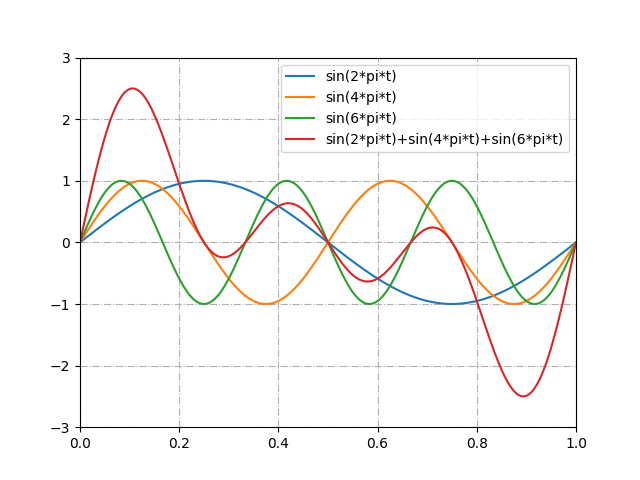
\includegraphics[width=0.4\textwidth]{assets/Figure_1.png}
	\caption{$\sin(2\cdot\pi\cdot t)+\sin(4\cdot\pi\cdot t)+\sin(8\cdot\pi\cdot t)$}
\end{figure}
\begin{enumerate}
	\item 一般表示为:
	      \begin{equation}\label{vtri}
		      f(t)=\sum\limits_{k=1}^n\ A_k\cdot \sin(2\cdot \pi\cdot k\cdot t+\phi_k)
	      \end{equation}

	      这里使用$\cos$也没有关系,但是这节课里就钦定了$\sin$。
	\item 由上图可以看出,整体的函数在周期最长的函数重复的时候才重复,可以说周期最长的函数奠定了整个函数的基调。$k=1​$时,$T=\frac{2\cdot \pi}{2\cdot \pi}=1​$,周期最长,所以$k=1​$的项被称为fundamental wave。而$k>1​$的项被称为harmonic wave。
\end{enumerate}

\section{傅立叶级数的两种表达方式}
\subsection{三角函数形式表示}
我们把\ref{vtri}展开:
\begin{align*}
	      & f(t)                                                                                                   \\
	=     & \sum\limits_{k=1}^n\ A_k\cdot \sin(2\cdot\pi\cdot k\cdot t+\phi_k)                                     \\
	=     & \sum\limits_{k=1}^n\ [A_k\cdot \sin(2\cdot\pi\cdot k\cdot t)                                           \\
	\cdot & \cos(\phi_k)+A_k\cdot \cos(2\cdot \pi\cdot k\cdot t)\cdot \sin(\phi_k)]                                \\
	=     & \sum\limits_{k=1}^n\ [a_k\cdot \sin(2\cdot\pi\cdot k\cdot t) +b_k\cdot \cos(2\cdot \pi\cdot k\cdot t)]
\end{align*}

其中:
$$
	\left\{
	\begin{array}{lr}
		a_k=A_k\cdot \cos(\phi_k) \\
		b_k=A_k\cdot \sin(\phi_k)
	\end{array}
	\right.
$$

所以我们得到:
\begin{equation}\label{vtrii}
	f(t) =\sum\limits_{k=1}^n\ [a_k\cdot \sin(2\cdot\pi\cdot k\cdot t) +b_k\cdot \cos(2\cdot \pi\cdot k\cdot t)]
\end{equation}
\subsection{复指形式表示}
因为根据\ref{vtrii}的展开,所以我们令(为什么这么令我也不知道,反正老师就是突然跳到这一步。他想怎么干就怎么干吧……):
\begin{equation}
	f(t)=\sum\limits_{k=-n}^n\ c_k\cdot e^{2\cdot \pi \cdot i \cdot k \cdot t}
\end{equation}

\section{傅立叶级数的对称性}
\subsection{欧拉公式Euler's Formula}
\begin{equation}
	e^{2\cdot \pi\cdot i\cdot k\cdot t} =  \cos(2\cdot \pi\cdot k\cdot t)+i\cdot \sin(2\cdot \pi\cdot k\cdot t)
\end{equation}
\begin{equation}
	\cos(2\cdot \pi\cdot k\cdot t)=\frac{e^{2\cdot \pi\cdot i\cdot k\cdot t+}+e^{-2\cdot \pi\cdot i\cdot k\cdot t}}{2}
\end{equation}
\begin{equation}
	\sin(2\cdot \pi\cdot k\cdot t)=\frac{e^{2\cdot \pi\cdot i\cdot k\cdot t+}-e^{-2\cdot \pi\cdot i\cdot k\cdot t}}{2\cdot i}
\end{equation}
\subsection{傅立叶级数的对称性}
假设​信号是一个实信号(real 信号),则信号中没有虚部,有​$f(t)=\overline {f(t)}$:
\begin{align*}
	  & f(t)                                                                                        \\
	= & \sum\limits_{k=-n}^n\ c_k\cdot e^{2\cdot \pi \cdot i \cdot k \cdot t}                       \\
	= & \overline{\sum\limits_{k=-n}^n\ c_k\cdot e^{2\cdot \pi \cdot i \cdot k \cdot t}}            \\
	= & \sum\limits_{k=-n}^n\ \overline{c_k}\cdot \overline{e^{2\cdot \pi \cdot i \cdot k \cdot t}} \\
	= & \sum\limits_{k=-n}^n\ \overline{c_k}\cdot e^{-2\cdot \pi \cdot i \cdot k \cdot t}
\end{align*}

因为$\sum\limits_{k=-n}^n=\sum\limits_{k=n}^{-n}$,所以把$k$变成$-k$,得:
\begin{align*}
	  & f(t)                                                                        \\
	= & \sum\limits_{k=-n}^n\ c_k\cdot e^{2\cdot \pi \cdot i \cdot k \cdot t}       \\
	= & \sum\limits_{-k=-n}^n\ c_{-k}\cdot e^{2\cdot \pi \cdot i \cdot k \cdot t}   \\
	= & \sum\limits_{k=n}^{-n}\ c_{-k}\cdot e^{-2\cdot \pi \cdot i \cdot k \cdot t} \\
	= & \sum\limits_{k=-n}^n\ c_{-k}\cdot e^{-2\cdot \pi \cdot i \cdot k \cdot t}
\end{align*}

由上面两个推导知:
$$
	f(x)=\sum\limits_{k=-n}^n \overline{c_k}\cdot e^{-2\cdot \pi \cdot i \cdot k \cdot t}=\sum\limits_{k=-n}^n c_{-k}\cdot e^{-2\cdot \pi \cdot i \cdot k \cdot t}
$$


所以得到:
\begin{equation}
	c_{-k}=\overline{c_k}
\end{equation}

那么我们可知:
\begin{align*}
	  & c_k\cdot e^{2\cdot \pi\cdot i\cdot k\cdot t}+c_{-k}\cdot e^{2\cdot \pi\cdot i\cdot (-k)\cdot t}                 \\
	= & c_k\cdot e^{2\cdot \pi\cdot i\cdot k\cdot t}+c_{-k}\cdot e^{-2\cdot \pi\cdot i\cdot k\cdot t}                   \\
	= & c_k\cdot e^{2\cdot \pi\cdot i\cdot k\cdot t}+\overline{c_k}\cdot e^{\overline{2\cdot \pi\cdot i\cdot k\cdot t}} \\
	= & c_k\cdot e^{2\cdot \pi\cdot i\cdot k\cdot t}+\overline{c_k\cdot e^{2\cdot \pi\cdot i\cdot k\cdot t}}            \\
	= & 2\cdot \Re\{C_k\cdot e^{2\cdot \pi \cdot i\cdot k\cdot t}\}
\end{align*}

所以$c_k\cdot e^{2\cdot \pi\cdot i\cdot k\cdot t}+c_{-k}\cdot e^{2\cdot \pi\cdot i\cdot (-k)\cdot t}$为一个实数。$\sum\limits_{k=-n}^n\ c_k\cdot e^{2\cdot \pi \cdot i \cdot k \cdot t}$可以表示一个实数。

\section{从三角函数到复指形}
\subsection{从三角函数到复指形}
\begin{align*}
	  & f(t)                                                                                                                      \\
	= & \sum\limits_{k=1}^n\ [a_k\cdot \sin(2\cdot\pi\cdot k\cdot t)                                                              \\
	+ & b_k\cdot \cos(2\cdot \pi\cdot k\cdot t)]+\frac{A_0}{2}                                                                    \\
	= & \sum\limits_{k=1}^n\ (a_k\cdot \frac{e^{2\cdot \pi\cdot i\cdot k\cdot t}- e^{-2\cdot \pi\cdot i\cdot k\cdot t}}{2\cdot i} \\
	+ & b_k\cdot \frac{e^{2\cdot \pi\cdot i\cdot k\cdot t+}+e^{-2\cdot \pi\cdot i\cdot k\cdot t}}{2})+\frac{A_0}{2}               \\
	= & \sum\limits_{k=1}^n\ (\frac{b_k-i\cdot a_k}{2}\cdot e^{2\cdot \pi\cdot i\cdot k\cdot t}                                   \\
	+ & \frac{b_k+i\cdot a_k}{2}\cdot e^{-2\cdot \pi\cdot i\cdot k\cdot t})+\frac{A_0}{2}
\end{align*}
设$c_0=\frac{1}{2}\cdot A_0$;$c_k=\frac{b_k-i\cdot a_k}{2}$;$c_{-k}=\overline{c_{k}}=\frac{b_k+i\cdot a_k}{2}$则:
\begin{align*}
	  & f(t)                                                                                                                          \\
	= & \sum\limits_{k=1}^n\ (c_k\cdot e^{2\cdot \pi\cdot k\cdot t}+c_{-k}\cdot e^{-2\cdot \pi\cdot k\cdot t})+c_0                    \\
	= & \sum\limits_{k=1}^n\ c_k\cdot e^{2\cdot \pi\cdot k\cdot t}+\sum\limits_{k=1}^n\ c_{-k}\cdot e^{-2\cdot \pi\cdot k\cdot t}+c_0 \\
	= & \sum\limits_{k=1}^n\ c_k\cdot e^{2\cdot \pi\cdot k\cdot t}+\sum\limits_{k=-1}^{-n}\ c_k\cdot e^{2\cdot \pi\cdot k\cdot t}+c_0 \\
	= & \sum\limits_{k=-n\ k\neq0}^n\ c_k\cdot e^{2\cdot \pi\cdot k\cdot t}+c_0
\end{align*}

为了表示一般的周期现象,光求$\sum\limits_{k=-n}^n$是不够的,我们必须考虑对周期信号进行无限项求和,即求:$\sum\limits_{k=-\infty}^\infty$。

We can use high frequencies to make sharp corners.
There is discontinuity in some high derivative that means that you are gonna have trouble repeating that phenomenon as a finite sum.
You are gonna have to make N layers and layers to represent it more and more accurately.

由于$\cos(x)$和$\sin(x)$是连续且无限可微分的,所以有限的$\cos(x)$或$\sin(x)$之和不能表示离散的函数或者不无限可微分的函数。
%TODO:c_0到底怎么解决???
所以最终:
\begin{equation}
	f(t)=\sum\limits_{k=-\infty}^\infty\ c_k\cdot e^{2\cdot \pi\cdot k\cdot t}+c_0
\end{equation}
\subsection{求解$c_k$}
我们由上面的推导可知:
\begin{align*}
	c_{-k} & =\overline{c_k}        \\
	c_0    & =c_{-0}=\overline{c_0}
\end{align*}

$f(t)=\sum\limits_{k=-\infty}^\infty c_k\cdot e^{2\cdot \pi \cdot i \cdot k \cdot t}$,取出其中任意一项$c_m\cdot e^{2\cdot \pi \cdot i\cdot m\cdot t} \quad m\in[-\infty,\infty]$:
\begin{align*}
	  & c_m                                                                                                                                                                 \\
	= & f(t)-\sum\limits_{k\neq m}^\infty c_k\cdot e^{2\cdot \pi\cdot i\cdot k\cdot t}                                                                                      \\
	= & e^{-2\cdot \pi \cdot i\cdot m\cdot t}\cdot f(t)-\sum\limits_{k\neq m}^\infty c_k\cdot e^{2\cdot \pi\cdot i\cdot m\cdot t}\cdot e^{-2\cdot \pi\cdot i\cdot k\cdot t} \\
	= & e^{-2\cdot \pi\cdot i\cdot m\cdot t}\cdot f(t)-\sum\limits_{k\neq m}^\infty c_k\cdot e^{2\cdot \pi\cdot i\cdot (k-m)\cdot t}
\end{align*}

对等式两边同时积分得到:
$$
	c_m=\int_0^1\ [e^{-2\cdot \pi\cdot i\cdot m\cdot t}\cdot f(t)-\sum\limits_{k\neq m}^\infty\ c_k\cdot e^{2\cdot \pi\cdot i\cdot (k-m)\cdot t}]\ dt
$$

因为$k\neq m$,所以$\int_0^1\ e^{2\cdot \pi\cdot i\cdot (k-m)\cdot t}\ dt=0$(该结论的证明后面有)。所以有:
$$
	c_m=\int_0^1 \ e^{-2\cdot \pi\cdot i\cdot m\cdot t}\cdot f(t)\ dt
$$

\subsection{傅立叶参数 傅立叶系数}
我们用新记号$\hat{f}(k)$表示$c_k$:
\begin{equation}
	\hat{f}(k)=\int_0^1 \ e^{-2\cdot \pi\cdot i\cdot m\cdot t}\cdot f(t)\ dt
\end{equation}

因为是傅立叶级数的项,所以变量为频率$k$。
傅立叶级数用以下方式表示:
\begin{equation}
	f(t)=\sum\limits_{k=-\infty}^\infty\ \hat{f}(k)\cdot e^{2\cdot \pi\cdot i\cdot k\cdot t }
\end{equation}

因为在时域中观察,所以变量为时间变量$t$。
这两个式子的指数中:
\begin{enumerate}
	\item $2\cdot \pi$为函数的周期。这个周期来自最初的三角函数的周期设定;
	\item $k​$为频域变量,在分析时域的时候作为常数处理;
	\item $t$为时域变量,在分析频域时作为常数处理。
\end{enumerate}
\section{通用性验证}
\subsection{适用范围}
\subsubsection{关于三角函数的讨论}
\begin{enumerate}
	\item 由于三角函数是连续的,因此有限项级数不能表示离散的函数;
	\item 由于三角函数是无限可微分的,因此有限项级数不能表示不无限可微分的函数。
\end{enumerate}


\subsubsection{Dirichlet Condition}
一个周期函数在任意一个周期内:
\begin{enumerate}
	\item 有有限个一类间断点;
	\item 有有限个极大值与极小值;
	\item 其绝对值可积。
\end{enumerate}

则可以表示为傅立叶级数。
\subsubsection{有限求和}
We can use high frequencies to make sharp corners. There is a discontinuity in some high derivative that means that you are going to have trouble repeating that phenomenon as a finite sum. You are going to take N layers and layers to try to represent it more and more accurately.
\subsection{收敛性}
为什么要讨论收敛?任何非平滑的信号都会产生无限多个傅立叶级数。如果在有限项后截断来得到函数近似,万一级数不收敛于$f(t)$,情况就很糟糕。
\subsubsection{$L_2$收敛}
一般信号(也包括上述两种情况)的收敛性在分析的时候,不采用逐点判断收敛性的方法,用均方收敛(convergence in the mean)。

如果$\int_{0}^{1}\ |f(t)|^2\ dt<\infty$,且:$\int_{0}^{1}\ |\sum\limits_{k=-n}^{n}\ \hat{f}(k)\cdot e^{-2\cdot \pi\cdot i\cdot k\cdot t\ dt-f(t)}|^2\rightarrow 0\ if\ n\rightarrow \infty$,则可表示为:
$$
	f\in L_2([0,1])
$$
\subsubsection{收敛结论}
\begin{enumerate}
	\item 如果信号是平滑连续的(连续可微),在所有的$t$处都会收敛于$f(t)$;
	\item 如果信号是有跳变的,在跳变点将收敛于跳变点前、后的平均值。
	      \begin{figure}[H]
		      \centering
		      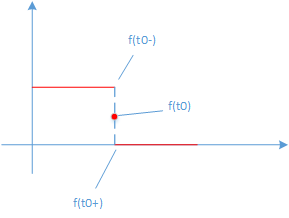
\includegraphics[width=0.4\textwidth]{assets/convergence.png}
		      \caption{跳变函数的收敛性}
	      \end{figure}
\end{enumerate}
\section{函数的内积}
\subsection{函数内积计算方法}
设有复变函数$f,g\in L_2([0,1])$,那么可以把$f,g$分别认为是Vector。求这两个Vector内积的方法为:
\begin{equation}
	(f,g)=\int_0^1\ f(t)\overline{g(t)}\ dt
\end{equation}
\begin{enumerate}
	\item $g(t)​$取共轭函数!!!!!
	\item 当$(f,g)=0$的时候,就可以说$f$与$g​$正交。
\end{enumerate}
\subsection{与Vector类比}
\begin{enumerate}
	\item 类比Vector的模:
	      $$
		      (f,f)=||f||^2=\int_0^1\ |f(t)|^2 \ dt
	      $$
	\item 当$f$与$g​$正交的时候,有函数形式的勾股定理:
	      $$
		      ||f+g||^2=||f||^2+||g||^2
	      $$
\end{enumerate}
\section{傅立叶级数与矩阵}
\subsection{空间内的Orthogonal Basis}
空间内一组标准正交向量:$q_1,q_2,\cdots ,q_n$。空间内任意向量$\mathbf{v}$有:
\begin{align*}
	v & =x_1\cdot q_1+x_2\cdot q_2+\cdots+x_n\cdot q_n=Q\cdot x \\
	x & =Q^{-1}\cdot v                                          \\
\end{align*}

因为$Q$为正交矩阵,所以$Q^T=Q^{-1}$,所以$x=Q^T\cdot v$。

因为$q_i$为标准Orthogonal Basis,所以$q_i^T\cdot q_j=0$。

所以$x_i=q_i^T\cdot v$。Vector与标准Orthogonal Basis的点乘,求得各分量。
\subsection{Orthogonal Basis}
\subsubsection{三角函数的Orthogonal Basis}
正弦余弦函数一定正交:
$$
	\int_0^{\frac{2\cdot \pi}{n}}\ \cos(n\cdot x)\sin(n\cdot x)=0
$$

相同频率的正弦函数不正交:
$$
	\int_0^{\frac{2\cdot \pi}{n}}\ \sin(n\cdot x)\sin(n\cdot x)=1
$$

相同频率的余弦函数不正交:
$$
	\int_0^{\frac{2\cdot \pi}{n}}\ \cos(n\cdot x)\cos(n\cdot x)=1
$$

由此性质,我们可以将$\sin(2\cdot \pi\cdot m \cdot t)$和$\cos(2\cdot \pi\cdot m \cdot t)$看作傅立叶级数上的Orthogonal Basis,來求解傅立叶系数。
\subsubsection{复指函数的Orthogonal Basis}
\begin{align*}
	  & (e^{2\cdot \pi\cdot i\cdot m\cdot t},e^{2\cdot \pi\cdot i\cdot n\cdot t})                      \\
	= & \int_0^1 \ e^{2\cdot \pi\cdot i\cdot m\cdot t}\cdot e^{2\cdot \pi\cdot i\cdot (-n)\cdot t}\ dt \\
	= & \int_0^1 \ e^{e^{2\cdot \pi\cdot i\cdot (m-n)\cdot t}}\ dt                                     \\
	= & \rsx{\frac{e^{2\cdot \pi\cdot i\cdot (m-n)\cdot t}}{2\cdot \pi \cdot i \cdot(m-n)}}_0^1
\end{align*}

展开$e^{2\cdot \pi\cdot i\cdot (m-n)\cdot t}$:
\begin{align*}
	  & e^{2\cdot \pi\cdot i\cdot (m-n)\cdot t}                                       \\
	= & \cos(2\cdot \pi \cdot t\cdot(m-n))+i \cdot \sin(2\cdot \pi \cdot t\cdot(m-n))
\end{align*}

因为$m,n\in \mathbb{Z}$,所以$m-n\in \mathbb{Z}$;所以$\cos(2\cdot \pi \cdot t\cdot(m-n))=1$;所以$\sin(2\cdot \pi \cdot t\cdot(m-n))=0$;所以$e^{2\cdot \pi\cdot i\cdot (m-n)\cdot t}-e^0=0$。

因此$e^{2\cdot \pi i\cdot k \cdot t}$被称为傅立叶变换中的Orthogonal Basis。
$$
	\begin{cases}
		(e^{2\cdot \pi\cdot i\cdot m\cdot t},e^{2\cdot \pi\cdot i\cdot m\cdot t}) & =1 \\
		(e^{2\cdot \pi\cdot i\cdot m\cdot t},e^{2\cdot \pi\cdot i\cdot n\cdot t}) & =0
	\end{cases}
$$
\subsection{求解傅立叶系数}
\subsubsection{三角函数形}
$f(t)$的三角函数表达式如下:

$$f(t)=\sum\limits_{k=1}^n\ [a_k\cdot \sin(2\cdot\pi\cdot k\cdot t) +b_k\cdot \cos(2\cdot \pi\cdot k\cdot t)]$$

将$f(t)$分别与$\sin(2\cdot \pi\cdot m \cdot t)$和$\cos(2\cdot \pi\cdot m \cdot t)$做内积,可以得到$a_m$和$b_m$:
\begin{align*}
	  & \int_0^1\ f(x)\cdot \sin(2\cdot \pi\cdot m \cdot t)\ dt            \\
	= & \int_0^1\ a_m\cdot \sin^2(2\cdot \pi\cdot m \cdot t)\ dt           \\
	= & \int_0^1\ a_m\cdot \frac{1-\cos(4\cdot \pi\cdot m \cdot t)}{2}\ dt \\
	= & \frac{a_m}{2}                                                      \\
\end{align*}
因此:
$$
	a_m=\frac{\int_0^1\ f(x)\cdot \sin(2\cdot \pi\cdot m \cdot t)\ dt}{\frac{1}{2}}
$$
同理:
$$
	b_m=\frac{\int_0^1\ f(x)\cdot \cos(2\cdot \pi\cdot m \cdot t)\ dt}{\frac{1}{2}}
$$
我们再来看看$c_m$:
\begin{align*}
	  & c_m                                                           \\
	= & \int_0^1 \ e^{-2\cdot \pi\cdot i\cdot m\cdot t}\cdot f(t)\ dt \\
	= & \int_0^1 \ [\cos(-2\cdot \pi\cdot i\cdot m\cdot t)            \\
	+ & i\cdot \sin(-2\cdot \pi\cdot i\cdot m\cdot t)\cdot f(t)]\ dt  \\
	= & \int_0^1 \ [\cos(2\cdot \pi\cdot i\cdot m\cdot t)             \\
	- & i\cdot \sin(2\cdot \pi\cdot i\cdot m\cdot t)\cdot f(t)]\ dt   \\
	= & \frac{b_m-i\cdot a_m}{2}
\end{align*}
与前面得到的结论一致。
\subsubsection{复指函数形}
如果$\mathbf{v}$是单位Vector,那么$(\mathbf{u},\mathbf{v})$是$\mathbf{u}$在$\mathbf{v}$上的投影。

类比到傅立叶级数:
\begin{align*}
	  & \hat{f}(k)                                                    \\                                          \\
	= & \int_0^1 \ f(t)\cdot e^{-2\cdot \pi\cdot i\cdot k\cdot t}\ dt \\
	= & (f(t),e^{2\cdot \pi\cdot i\cdot k\cdot t})
\end{align*}

因此傅立叶系数\ $\hat{f}(k)$是原函数$f(t)$在$e^{-2\cdot \pi\cdot i\cdot k\cdot t}$上的投影。

几何上的分量:
$$
	\mathbf{a}_{\mathbf{v}}=(\mathbf{a},\mathbf{v})\cdot \mathbf{v}
$$
\begin{enumerate}
	\item 先通过内积得到投影;
	\item 然后用投影乘上代表Vector方向的Orthogonal Basis得到该方向上的分量。
\end{enumerate}

类比到傅立叶级数:
\begin{align*}
	  & f(t)                                                                                                             \\
	= & \sum\limits_{k=-\infty}^\infty \ \hat{f}(t)\cdot e^{2\cdot \pi\cdot i\cdot k\cdot t}                             \\
	= & \sum\limits_{k=-\infty}^\infty\ (f,e^{2\cdot \pi\cdot i\cdot k\cdot t})\cdot e^{2\cdot \pi\cdot i\cdot k\cdot t}
\end{align*}

\begin{enumerate}
	\item 函数进行傅立叶级数后的每一项,都是函数在不同的Orthogonal Basis$e^{2\cdot \pi\cdot i\cdot k\cdot t}$上的分量。
	\item 反过来,这些分量相加构成完整的原始函数。
\end{enumerate}

下面补充Rayleigh's Identity。几何上,因为$\mathbf{c}^2=\mathbf{a}^2+\mathbf{b}^2$,所以$(\mathbf{a},\mathbf{b})=0$。类比到傅立叶级数,帕塞瓦尔定理的定义如下:
$$
	\int_0^1\ |f(t)|^2\ dt=\sum\limits_{k=-\infty}^{\infty}\ |\hat{f}(x)|^2
$$

傅立叶变换后的项互为正交项,正交项内积为$0$。
\section{卷积}
It is 卷积 in time, multiplication in 频率.

一般来说,频域的运算会比时域简单许多,因为频域只需执行相乘运算。
\subsection{定义}
设$f(t)$、$g(t)$是$\mathbb{R}$上两个可积函数,作积分:
$$
	\int_{-\infty}^\infty\ f(\tau)\cdot g(t-\tau)\ d\tau
$$
可以证明,关于几乎所有的 $x\in (-\infty ,\infty )$,上述积分是存在的。这样,随着$x$的不同取值,这个积分就定义了一个新函数$h(x)$,称为函数$f$与$g$的卷积,记为:
$$
	h(x)=(f*g)(t)=\int_{-\infty}^{\infty}\ f(r)\cdot g(t-r)\ dr
$$
\subsection{卷积与偏微分方程}
偏微分方程的解经常以卷积的形式出现。卷积的一方是特解,另一方是给定的初始数据下的初始条件。
\subsection{图解卷积}
\begin{figure}[H]
	\centering
	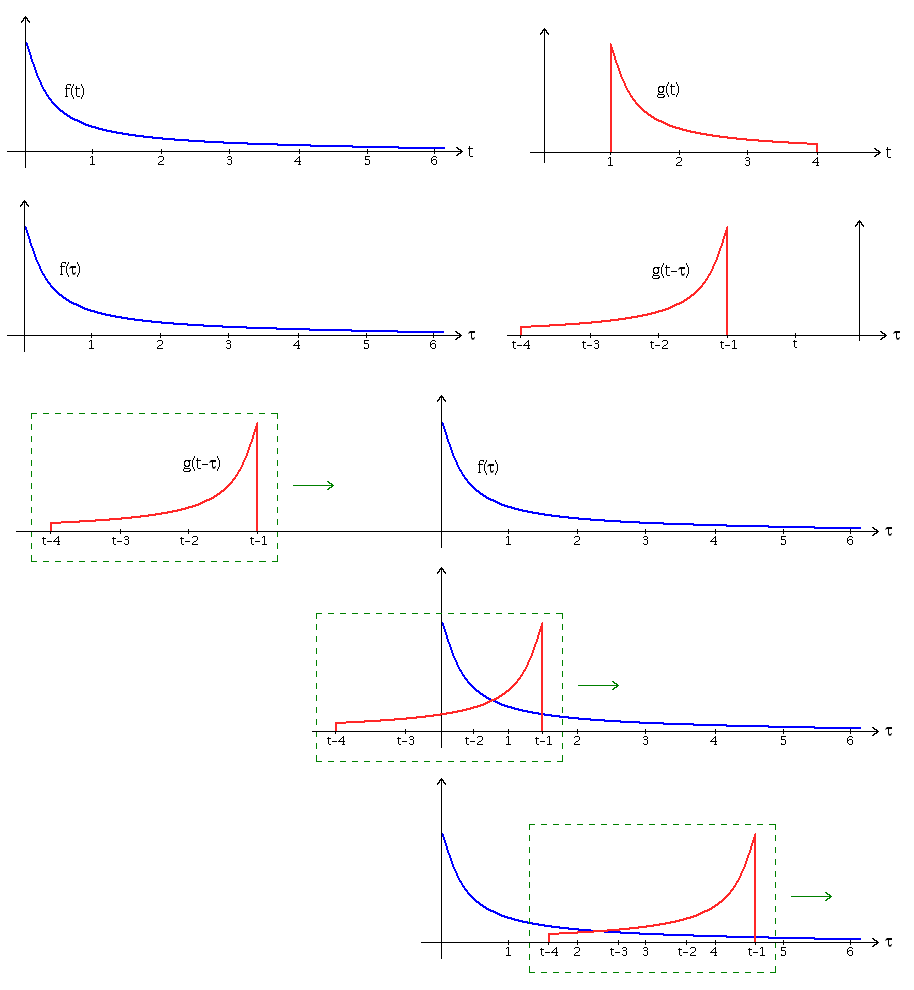
\includegraphics[width=0.4\textwidth]{assets/Convolution.png}
	\caption{图解卷积}
\end{figure}

\begin{enumerate}
	\item 已知两函数$f(t)$和$g(t)$。上图第一行分别为$f(t)$和$g(t)$。
	\item 首先将两个函数都用$\tau$来表示,从而得到$f(\tau)$和$g(\tau)$。将函数$g(\tau)$向右移动t个单位,得到函数$g(\tau-t)$的图像。将$g(\tau-t)$翻转至纵轴另一侧,得到$g(t-\tau)$的图像。上图第二行两图分别为$f(\tau)$和$g(t-\tau)$。
	\item 由于$\tau$是时间变量,当时间变量(以下简称“时移”)取不同值时,$g(t-\tau)$能沿着$\tau$轴“滑动”。右图第三四五行可理解为“滑动”。
	\item 让$\tau$从$-∞$滑动到$+∞$。两函数交会时,计算交会范围中两函数乘积的积分值。换句话说,我们是在计算一个滑动的的加权总和。也就是使用$g(t-\tau )$当做加权函数,来对$f(\tau)$取加权值。
	\item 最后得到的波形(未包含在此图中)就是$f$和$g$的卷积。如果$f(t)$是一个单位脉冲,我们得到的乘积就是$g(t)$本身,称为冲激响应。
\end{enumerate}
\section{从Fourier Series到Fourier Transform}
我们将非周期函数看作是周期函数的一种特殊情况:周期趋向无穷。
\subsection{对于周期为1的函数}
\begin{align*}
	c_k=\hat{f}(k)=\int_0^1\ e^{-2\cdot \pi\cdot i\cdot k\cdot t}\cdot f(t)\ dt \\
	f(t)=\sum\limits_{k=-\infty}^{\infty}\ \hat{f}(k)\cdot e^{2\cdot \pi\cdot i\cdot k\cdot t}
\end{align*}
\begin{figure}[H]
	\centering
	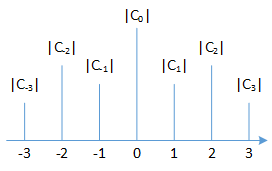
\includegraphics[width=0.4\textwidth]{assets/ft1.png}
	\caption{周期为$1$的函数是频谱图。由于$c_k$为复数形式,因此我们无法在图上画出,因此只能画出$c_k$的模。另外我们在第二节课的时候也学过,$c_k$是$y$轴对称的。}
\end{figure}
\begin{enumerate}
	\item Fourier Transform是对Fourier Coefficient的一般化;
	\item Inverse Fourier Transform是对Fourier Series的一般化。
\end{enumerate}
\subsection{对于周期为T的函数}
$$
	c_k=\frac{1}{T}\cdot \int_{-\frac{T}{2}}^{\frac{T}{2}}\ e^{-2\cdot \pi\cdot i\cdot \frac{k}{T}\cdot t}\cdot f(t)\ dt
$$
$$
	f(t)=\sum\limits_{k=-\infty}^{\infty}\ \hat{f}(k)\cdot e^{2\cdot \pi\cdot i\cdot\cdot  \frac{k}{T}\cdot t}
$$

\begin{figure}[H]
	\centering
	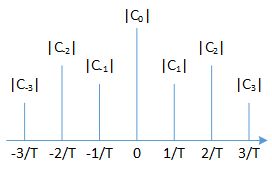
\includegraphics[width=0.4\textwidth]{assets/ft2.png}
	\caption{周期为$T$的函数的频谱图。由于周期为$T$,因此频率为$\frac{1}{T}$。当$T\rightarrow\infty$时,$\frac{1}{T}\rightarrow 0$,此时频谱会变得连续了。}
\end{figure}
\begin{enumerate}
	\item 这里为什么有个$\frac{1}{T}$???老师说从头开始推,他就不推了,你可以推推。
	\item 对于周期函数来说,积分的周期从哪里开始到哪里结束没人在意。
\end{enumerate}
\subsection{对于周期为$\infty$的函数}
只让$T\rightarrow \infty$不能得到Fourier Transform:
\begin{figure}[H]
	\centering
	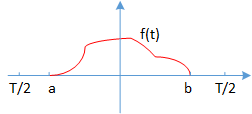
\includegraphics[width=0.4\textwidth]{assets/ft3.png}
	\caption{周期为$\infty$的函数的频谱图}
\end{figure}
\begin{align*}
	     & \hat{f}(k)                                                                                                       \\
	=    & \frac{1}{T}\cdot \int_{-\frac{T}{2}}^{\frac{T}{2}}\ e^{-2\cdot \pi\cdot i\cdot \frac{k}{T}\cdot t}\cdot f(t)\ dt \\
	=    & \frac{1}{T}\cdot \int_{a}^{b}\ e^{-2\cdot \pi\cdot i\cdot \frac{k}{T}\cdot t}\cdot f(t)\ dt                      \\
	\leq & \frac{1}{T}\cdot \int_{a}^{b}\ |e^{-2\cdot \pi\cdot i\cdot \frac{k}{T}\cdot t}|\cdot |f(t)|\ dt                  \\
	=    & \frac{1}{T}\cdot \int_{a}^{b}\ Mod\{[\cos^2(-2\cdot \pi\cdot i\cdot \frac{k}{T}\cdot t)                          \\
	+    & \sin^2(-2\cdot \pi\cdot i\cdot \frac{k}{T}\cdot t)]^{\frac{1}{2}}\}\cdot |f(t)|\ dt                              \\
	=    & \frac{1}{T}\cdot \int_a^b 1\cdot |f(t)|\ dt                                                                      \\
	=    & \frac{M}{T}
\end{align*}
即对所有$c_k=\hat{f}(k)$都有:$c_k\leq \frac{M}{T}$。

$M$是该函数绝对值的积分,是有限值。如果$T\rightarrow \infty$,那么$c_k\rightarrow 0$;则所有Fourier Coefficient全都没有意义。
\section{新符号$\mathcal{F}$}
由于$c_k\leq \frac{M}{T}$,$c_k$和$T$成反比,所以我们想到把$T$和$c_k$相乘,这样就不会出现上面的问题了。

在Fourier Series中,$\mathcal{F}f(k)=c_k$,现在令$\mathcal{F}f(\frac{k}{T})=c_k\cdot T$,这是Fourier Transform线性的一种体现。

\begin{align*}
	     & \mathcal{F}f(\frac{k}{T})   =    c_k\cdot T                                                                                      \\
	=    & \int_{-\frac{T}{2}}^{\frac{T}{2}}\ e^{-2\cdot \pi\cdot i\cdot \frac{k}{T}\cdot t}\cdot f(t)\ dt                                  \\
	f(t) & =\sum\limits_{k=-\infty}^{\infty}\ \mathcal{F}f(\frac{k}{T})\cdot e^{2\cdot \pi\cdot i\cdot \frac{k}{T}\cdot t}\cdot \frac{1}{T}
\end{align*}

取值间隔为$\frac{1}{T}\rightarrow 0$,趋于连续变量,现在用连续变量$s$来表示$\frac{k}{T}$:
\begin{align*}
	  & \mathcal{F}f(s)                                                                       \\
	= & c_k\cdot T                                                                            \\
	= & \int_{-\frac{T}{2}}^{\frac{T}{2}}\ e^{-2\cdot \pi\cdot i\cdot s\cdot t}\cdot f(t)\ dt \\
	= & \int_{-\infty}^{\infty}\ e^{-2\cdot \pi\cdot i\cdot s\cdot t}\cdot f(t)\ dt
\end{align*}
由于$\frac{k}{T}$被替换为连续变量$s$,因此Fourier Series中的多项式之和被替换成积分,其中$\frac{1}{T}$为$\Delta s$,即$ds$:
\begin{align*}
	f(t)   =  \int_{-\infty}^{\infty}\ \mathcal{F}f(s)\cdot e^{2\cdot \pi\cdot i\cdot s\cdot t}\ ds
\end{align*}
\section{Fourier Transform和Inverse Fourier Transform}
\subsection{Fourier Transform}
\subsubsection{两种书写方式}
\begin{enumerate}
	\item $\mathcal{F}f(s)=\int_{-\infty}^{\infty}\ e^{-2\cdot \pi\cdot i\cdot s\cdot t}\cdot f(t)\ dt$;
	\item $F(s)=\int_{-\infty}^{\infty}\ e^{-2\cdot \pi\cdot i\cdot s\cdot t}\cdot f(t)\ dt$。
\end{enumerate}
\subsubsection{注解}
Fourier Transform在Frequency Domain上分析Signal,因此自变量为频率变量$s$。
\subsection{Inverse Fourier Transform}
\subsubsection{两种书写方式}
\begin{enumerate}
	\item $\mathcal{F}^{-1}g(s)=\int_{-\infty}^{\infty}\ g(s)\cdot e^{2\cdot \pi\cdot i\cdot s\cdot t}\ ds$;
	\item $f(t)=\int_{-\infty}^{\infty}\ \mathcal{F}f(s)\cdot e^{2\cdot \pi\cdot i\cdot s\cdot t}\ ds$。
\end{enumerate}
\subsubsection{注解}
Inverse Fourier Transform在Time Domain上分析Signal,因此自变量为时间变量$t$。
\subsection{Fourier Transform和Inverse Fourier Transform之间的关系}
\begin{enumerate}
	\item $\mathcal{F}^{-1}\mathcal{F}f=f$
	\item $\mathcal{F}\mathcal{F}^{-1}g=g$
\end{enumerate}
\subsection{零点的值}
\begin{align*}
	\mathcal{F}f(0)      & =\int_{-\infty}^{\infty}\ e^{-2\cdot \pi\cdot i\cdot 0\cdot t}\cdot f(t)\ dt=\int_{-\infty}^{\infty}\ f(t)\ dt \\
	\mathcal{F}^{-1}g(0) & =\int_{-\infty}^{\infty}\ e^{-2\cdot \pi\cdot i\cdot s\cdot 0}\cdot g(s)\ ds=\int_{-\infty}^{\infty}\ g(s)\ ds
\end{align*}
\section{Fourier Transform实例}
\subsection{$\Pi$函数}
$$
	\pi(t)=
	\begin{cases}
		1 & |t|\leq\frac{1}{2} \\
		0 & |t|\geq\frac{1}{2}
	\end{cases}
$$
\begin{figure}[H]
	\centering
	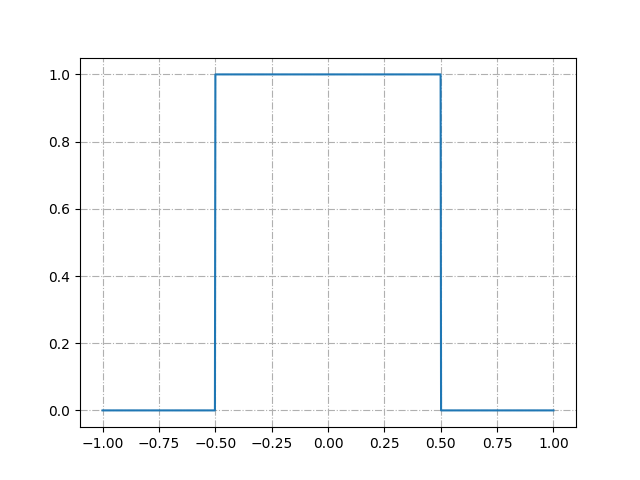
\includegraphics[width=0.4\textwidth]{assets/Figure_3.png}
	\caption{$\Pi$函数}
\end{figure}
\begin{align*}
	  & \mathcal{F}\ \Pi(s)                                                                                                            \\
	= & \int_{-\infty}^{\infty}\ e^{-2\cdot \pi\cdot i\cdot s\cdot t}\cdot \Pi(t)\ dt                                                  \\
	= & \rsx{-\frac{1}{2\cdot\pi\cdot i\cdot s}\cdot e^{-2\cdot \pi\cdot i\cdot s\cdot t}}_{-\frac{1}{2}}^{\frac{1}{2}}                \\
	= & -\frac{1}{2\cdot\pi\cdot i\cdot s}\cdot e^{- \pi\cdot i\cdot s}+\frac{1}{2\cdot\pi\cdot i\cdot s}\cdot e^{- \pi\cdot i\cdot s} \\
	= & \frac{1}{\pi\cdot s}\cdot \frac{e^{\pi\cdot i\cdot s}-e^{- \pi\cdot i\cdot s}}{2\cdot i}                                       \\
	= & \frac{\sin(\pi\cdot s)}{\pi\cdot s}                                                                                            \\
	= & \sinc(\pi\cdot s)
\end{align*}
\begin{figure}[H]
	\centering
	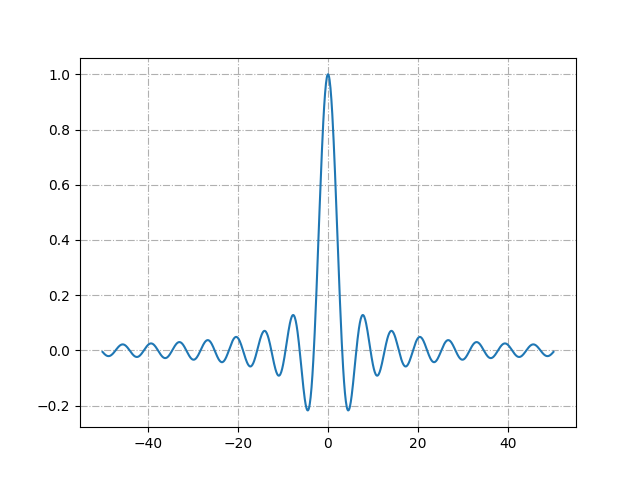
\includegraphics[width=0.4\textwidth]{assets/Figure_2.png}
	\caption{$\sinc$函数}
\end{figure}
\subsection{$\Lambda$函数}
\begin{figure}[H]
	\centering
	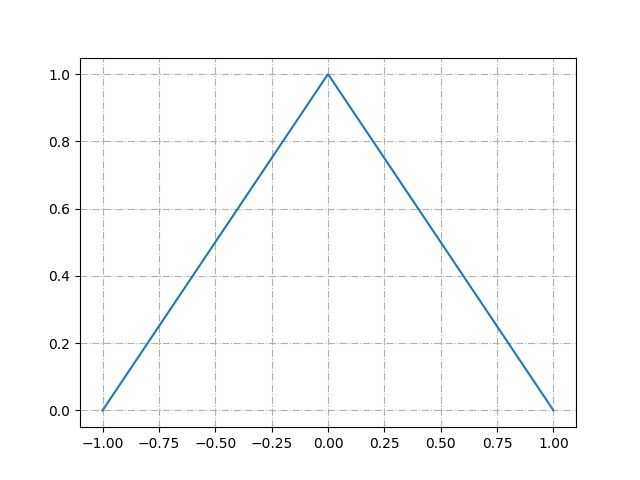
\includegraphics[width=0.4\textwidth]{assets/Figure_4.png}
	\caption{$\Lambda$函数}
\end{figure}
\begin{align*}
	  & \mathcal{F}\ \Lambda(s)                                                                                                              \\
	= & \int_{-\infty}^{\infty}\ e^{-2\cdot \pi\cdot i\cdot s\cdot t}\cdot \Lambda(t)\ dt                                                    \\
	= & \int_{-1}^{0}\ e^{-2\cdot \pi\cdot i\cdot s\cdot t}\cdot (1+t)\ dt+\int_{0}^{1}\ e^{-2\cdot \pi\cdot i\cdot s\cdot t}\cdot (1-t)\ dt \\
	= & \frac{\cos^2(\pi\cdot s)}{\pi\cdot s}                                                                                                \\
	= & \sinc^2(\pi\cdot s)
\end{align*}
\subsection{$\Lambda$与$\Pi$之间的关系}
Every Signal has a spectrum, the spectrum determines the Signal.

我们可以看到$\Pi$函数和$\Lambda$函数经过Fourier Transform后奇妙的平方关系。事实上,通过后面利用Fourier Transform证明大数定律可知,任何Signal经过几次Fourier Transform之后的频谱图都会变得越来越像一个“钟形”,即正态分布的样子。往后看一看Convolution相关的知识可以看到:
$$
	\mathcal{F}f(\pi*\pi)=(\mathcal{F}f\ \pi)\cdot(\mathcal{F}f\ \pi)=\sinc^2=\mathcal{F}\ \Lambda
$$

一般情况下,$f*g$都比单独的$f$或$g$要平滑一些。就好像矩形函数$\Pi$没有三角函数$\Lambda$平滑一些。
\section{Fourier Transform的对称性}
\subsection{Time Domain和Frequency Domain之间的对称关系}
\begin{enumerate}
	\item Fourier Transform从Time Domain转换到Frequency Domain;
	\item Inverse Fourier Transform从Frequency Domain转换到Time Domain。
\end{enumerate}
\subsection{反转Signal}
令$f^-(t)=f(-t)$,$f^-(t)$即为$f(t)$的反转。

\subsection{对偶定理}
\subsubsection{对偶定理1}
由反转函数的定义得:
$$
	\mathcal{F}f(-s)=(\mathcal{F}f)^-(s)
$$

又因为:
\begin{align*}
	  & \mathcal{F}f(-s)                                                           \\
	= & \int_{-\infty}^{\infty}\ e^{2\cdot \pi\cdot i\cdot s\cdot t}\cdot f(t)\ dt \\
	= & \mathcal{F}^{-1}f(s)
\end{align*}

所以:
\begin{equation}\label{du1}
	(\mathcal{F}f)^-=\mathcal{F}^{-1}f
\end{equation}

函数Fourier Transform的反转等于对该函数进行Inverse Fourier Transform。

在积分中,变量叫什么不重要。在\eqref{du1}中,积$s$和积$t$是一样的效果。

Fourier Transform的变量是Frequency Domain变量$s$。

$\mathcal{F}^{-1}f$中对Time Domain进行了Inverse Fourier Transform。And this makes no sense. But, math is math, nobody cares.

\subsubsection{对偶定理2}
\begin{align*}
	  & \mathcal{F}(f^-(t))                                                                            \\
	= & \int_{-\infty}^{\infty}\ e^{-2\cdot \pi\cdot i\cdot s\cdot t}\cdot f(-t)\ dt                   \\
	= & \int_{\infty}^{-\infty}\ e^{-2\cdot \pi\cdot i\cdot s\cdot (-u)}\cdot f(u)\ d(-u) \quad (u=-t) \\
	= & \int_{-\infty}^{\infty}\ e^{2\cdot \pi\cdot i\cdot s\cdot u}\cdot f(u)\ du                     \\
	= & \mathcal{F}^{-1}f(u)
\end{align*}
\begin{equation}\label{du2}
	\mathcal{F}(f^-)=\mathcal{F}^-f
\end{equation}

函数反转的Fourier Transform等于对该函数进行Inverse Fourier Transform。

\eqref{du1}与\eqref{du2}的不同之处在于,\eqref{du1}是在Frequency Domain上进行讨论,\eqref{du2}是在Time Domain上进行讨论。
\subsubsection{对偶定理3}
由\eqref{du1}和\eqref{du2}得:
\begin{equation}\label{du3}
	(\mathcal{F}f)^-=\mathcal{F}(f^-)
\end{equation}

由函数的Fourier Transform的反转等于该函数Fourier Transform的逆变换及该函数反转的Fourier Transform等于Fourier Transform的逆变换得出函数反转的Fourier Transform等于函数Fourier Transform的反转。
\subsubsection{对偶定理4}
\begin{equation}
	\mathcal{F}\mathcal{F}f= \mathcal{F}(\mathcal{F}f)=\mathcal{F}(\mathcal{F}^-(f^-)) =  f^-
\end{equation}

函数连续进行两次傅里叶变换等于该函数的反转。

我们可以看一个应用:
\begin{align*}
	\because   & \mathcal{F}\Pi=\sinc                                 \\
	\therefore & \mathcal{F}\sinc=\mathcal{F}\mathcal{F}\Pi=\Pi^-=\Pi
\end{align*}

\section{Fourier Transform的时延性}
Shift in time corresponds to a phase shift in frequency.

Time Domain上的时移对应Frequency Domain上的相移:
\begin{align*}
	  & \int_{-\infty}^{\infty}\ e^{-2\cdot \pi\cdot i\cdot s\cdot t}\cdot f(t-b)\ dt                                         \\
	= & \int_{-\infty}^{\infty}\ e^{-2\cdot \pi\cdot i\cdot s\cdot (u+b)}\cdot f(u)\ du\quad (u=t-b)                          \\
	= & \int_{-\infty}^{\infty}\ e^{-2\cdot \pi\cdot i\cdot s\cdot u}\cdot e^{-2\cdot \pi\cdot i\cdot s\cdot b}\cdot f(u)\ du \\
	= & e^{-2\cdot \pi\cdot i\cdot s\cdot b}\cdot \int_{-\infty}^{\infty}\ e^{-2\cdot \pi\cdot i\cdot s\cdot u}\ du           \\
	= & e^{-2\cdot \pi\cdot i\cdot s\cdot b}\cdot \mathcal{F}f(s)                                                             \\
\end{align*}


如果原始Signal为$f(t)$,其Fourier Transform为$\mathcal{F}f(s)$;

如果原始Signal为$f(t\pm b)$,其Fourier Transform为$e^{\pm 2\cdot \pi\cdot i\cdot s\cdot b}\cdot \mathcal{F}f(s)$:
\begin{equation}
	\mathcal{F}[f(t\pm b)](s)=e^{\pm 2\cdot \pi\cdot i\cdot s\cdot b}\cdot \mathcal{F}f(s)
\end{equation}

Fourier Transform得到一个复数,包括幅度和相位。我们可以将$\mathcal{F}f(s)$表示成:
$$
	\mathcal{F}f(s)=|\mathcal{F}f(s)|\cdot e^{2\cdot \pi\cdot i\cdot \theta(s)}
$$

其中$|\mathcal{F}|$表示振幅,$\theta(s)$表示相位,那么:
\begin{align*}
	  & e^{-2\cdot \pi\cdot i\cdot s\cdot b}\cdot \mathcal{F}f(s)                      \\
	= & |\mathcal{F}f(s)|\cdot e^{-2\cdot \pi\cdot i\cdot s\cdot (\theta(s)-s\cdot b)}
\end{align*}


上面的等式代表了频谱的振幅不变,而相位改变了。

\section{Fourier Transform的尺度变化}
\begin{quote}
	下面之所以讨论$a$的正负性是因为正负性对积分上下界有影响。
\end{quote}
\subsection{证明}
\subsubsection{$a>0$时}
\begin{align*}
	  & \int_{-\infty}^{\infty}\ e^{-2\cdot \pi\cdot i\cdot s\cdot t}\cdot f(a\cdot t)\ dt                          \\
	= & \int_{-\infty}^{\infty}\ e^{-2\cdot \pi\cdot i\cdot s\cdot \frac{u}{a}}f(u)\ d\frac{u}{a}\quad (u=a\cdot t) \\
	= & \frac{1}{a}\cdot \int_{-\infty}^{\infty}\ e^{-2\cdot \pi\cdot i\cdot \frac{s}{a}\cdot u}\cdot f(u)\ du      \\
	= & \frac{1}{a}\cdot \mathcal{F}f(\frac{s}{a})
\end{align*}
\subsubsection{$a<0$时}
\begin{align*}
	  & \int_{-\infty}^{\infty}\ e^{-2\cdot \pi\cdot i\cdot s\cdot t}\cdot f(a\cdot t)\ dt                          \\
	= & \int_{-\infty}^{\infty}\ e^{-2\cdot \pi\cdot i\cdot s\cdot \frac{u}{a}}f(u)\ d\frac{u}{a}\quad (u=a\cdot t) \\
	= & \frac{1}{a}\cdot \int_{\infty}^{-\infty}\ e^{-2\cdot \pi\cdot i\cdot \frac{s}{a}\cdot u}\cdot f(u)\ du      \\
	= & -\frac{1}{a}\cdot \int_{-\infty}^{\infty}\ e^{-2\cdot \pi\cdot i\cdot \frac{s}{a}\cdot u}\cdot f(u)\ du     \\
	= & -\frac{1}{a}\cdot \mathcal{F}f(\frac{s}{a})
\end{align*}
\subsubsection{总结}
$$
	f(a\cdot t)\leftrightarrow \frac{1}{|a|}\cdot \mathcal{F}f(\frac{t}{a})
$$
\subsection{注解}
\begin{enumerate}
	\item Time Domain和Frequency Domain不可能同时在一个方向上压缩与拓展。
	\item Heidenberg 测不准原理
	      不能在空间和时间同时定位一个粒子;也不能同时任意精确地知道物体的速度和位置。这个定理是通过Fourier Transform来证明的。
\end{enumerate}
\section{Fourier Transform的Convolution}
Signal处理可以被理解为:如何用一个函数(Signal)调制另一个函数(Signal)。

Signal Processing can be said to how can you use one function(Signal) to modify another.

大部分情况下,Signal处理是着力于改变Signal的频谱,也就是说,先对Signal进行傅里叶变换,然后在Frequency Domain进行处理,之和进行傅里叶逆变换得到处理过后的Signal。
\subsection{线性处理}
\begin{align*}
	  & \mathcal{F}(f+g)                                                                                                                                        \\
	= & \int_{-\infty}^{\infty}\ e^{-2\cdot \pi\cdot i\cdot s\cdot t}\cdot [f(t)+g(t)]\ dt                                                                      \\
	= & \int_{-\infty}^{\infty}\ [e^{-2\cdot \pi\cdot i\cdot s\cdot t}\cdot f(t)+e^{-2\cdot \pi\cdot i\cdot s\cdot t}\cdot g(t)]\ dt                            \\
	= & \int_{-\infty}^{\infty}\ e^{-2\cdot \pi\cdot i\cdot s\cdot t}\cdot f(t)\ dt+\int_{-\infty}^{\infty}\ e^{-2\cdot \pi\cdot i\cdot s\cdot t}\cdot g(t)\ dt \\
	= & \mathcal{F}f+\mathcal{F}g
\end{align*}
如果对$f$的频谱不满意,可以用$g$进行调制。通过叠加$g$的频谱对Signal进行处理。
\subsection{Frequency Domain相乘处理}
\begin{align*}
	  & \mathcal{F}f\cdot \mathcal{F}g                                                                                                                               \\
	= & \int_{-\infty}^{\infty}\ e^{-2\cdot \pi\cdot i\cdot s\cdot t}\cdot g(t)\ dt\cdot \int_{-\infty}^{\infty}\ e^{-2\cdot \pi\cdot i\cdot s\cdot x}\cdot f(x)\ dx \\
	= & \iint_{-\infty}^{\infty}\ e^{-2\cdot \pi\cdot i\cdot s\cdot t}\cdot e^{-2\cdot \pi\cdot i\cdot s\cdot x}\cdot g(t)\cdot f(x)\ dt\ dx                         \\
	= & \int_{-\infty}^{\infty}\ [\int_{-\infty}^{\infty}\ e^{-2\cdot \pi\cdot i\cdot s\cdot (t+x)}\cdot g(t)\ dt]\cdot f(x)\ dx                                     \\
	= & \int_{-\infty}^{\infty}\ [\int_{-\infty}^{\infty}\ e^{-2\cdot \pi\cdot i\cdot s\cdot u}\cdot g(u-x)\ du]\cdot f(x)\ dx                                       \\
	  & (u=t+x)                                                                                                                                                      \\
	= & \int_{-\infty}^{\infty}\ [\int_{-\infty}^{\infty}\ g(u-x)\cdot f(x)\ dx]e^{-2\cdot \pi\cdot i\cdot s\cdot u}\ du                                             \\
\end{align*}
令$h(u)=\int_{-\infty}^{\infty}\ g(u-x)\cdot f(x)\ dx$,那么:
\begin{align*}
	\mathcal{F}g\cdot \mathcal{F}f=\int_{-\infty}^{\infty}\ e^{-2\cdot \pi\cdot i\cdot s\cdot u}\cdot h(u)\ du
\end{align*}

Signal的Convolution的Fourier Transform等于对这些Signal进行Fourier Transform后的Convolution。
\begin{equation}
	\mathcal{F}(g*f)=(\mathcal{F}g)\cdot(\mathcal{F}f)
\end{equation}

I think it is equally idiotic to try to visualize convolution. I think the way to visualize convolution if there is a way, is to think in terms of multiplying in the frequency domain.
\section{滤波}
一般人会把Convolution和滤波混为一谈,但实际上,Convolution是滤波的Convolution(比如低通滤波算Convolution,高通滤波就不算Convolution)。
\subsection{滤波器}
是一个输入可变的函数(Signal)与一个固定的函数(Signal)进行Convolution运算的系统。这个固定的Signal叫做脉冲响应(impulse response)。
\begin{align*}
	 & g      & = & f     & * & h                 \\
	 & output & = & input & * & impulse\ response
\end{align*}

$$
	\mathcal{F}g(s)=\mathcal{F}f(s)\cdot \mathcal{F}h(s)
$$
$\mathcal{F}f(s)$被称为传递函数(Transfer Function)。在设计滤波器的时候通常是设计合适的$\mathcal{F}f(s)$。
\subsection{常见滤波器}
\begin{figure}[H]
	\centering
	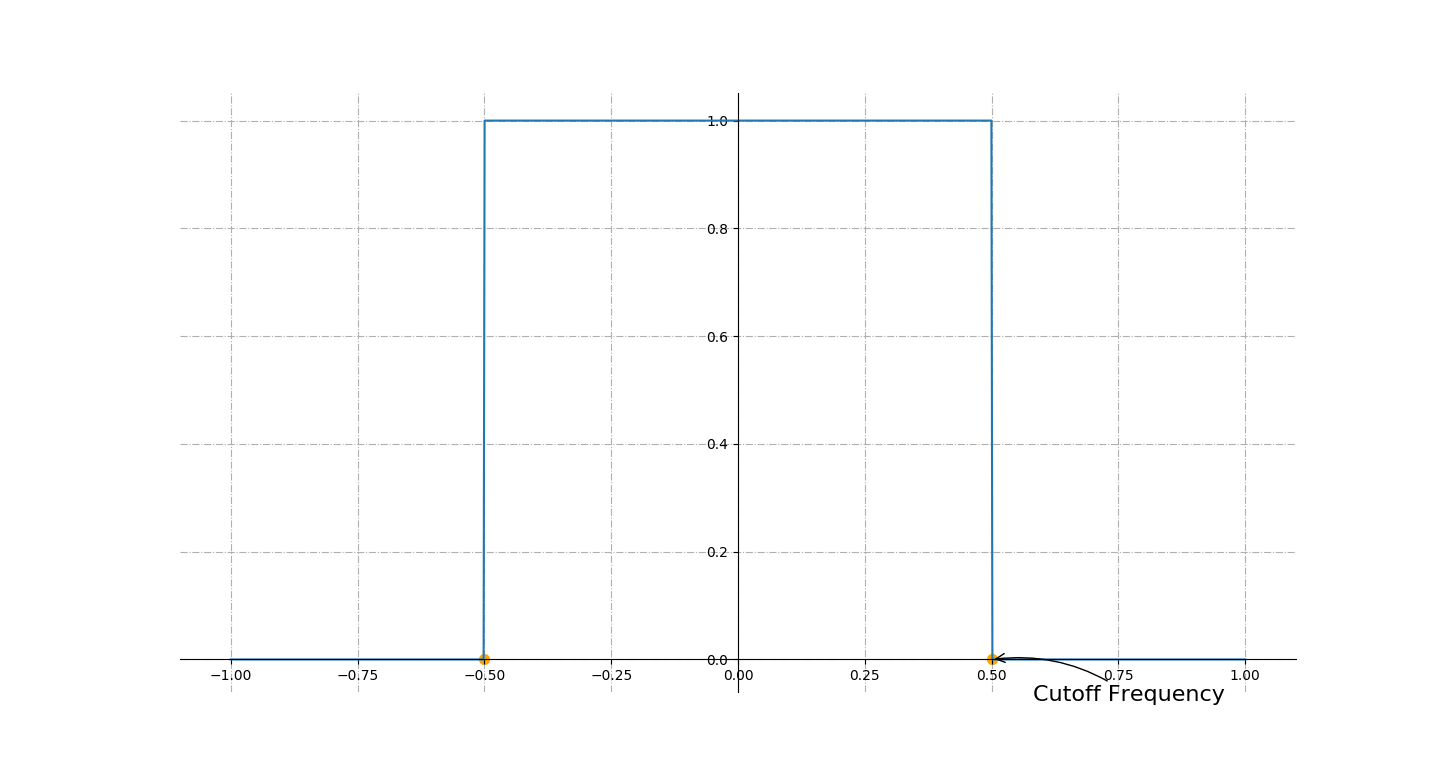
\includegraphics[width=0.4\textwidth]{assets/Figure_5.png}
	\caption{低通滤波器(Low Pass Filter):在Time Domain中的结果相当于与一个特定的$\sinc$函数进行Convolution。}
\end{figure}
\begin{figure}[H]
	\centering
	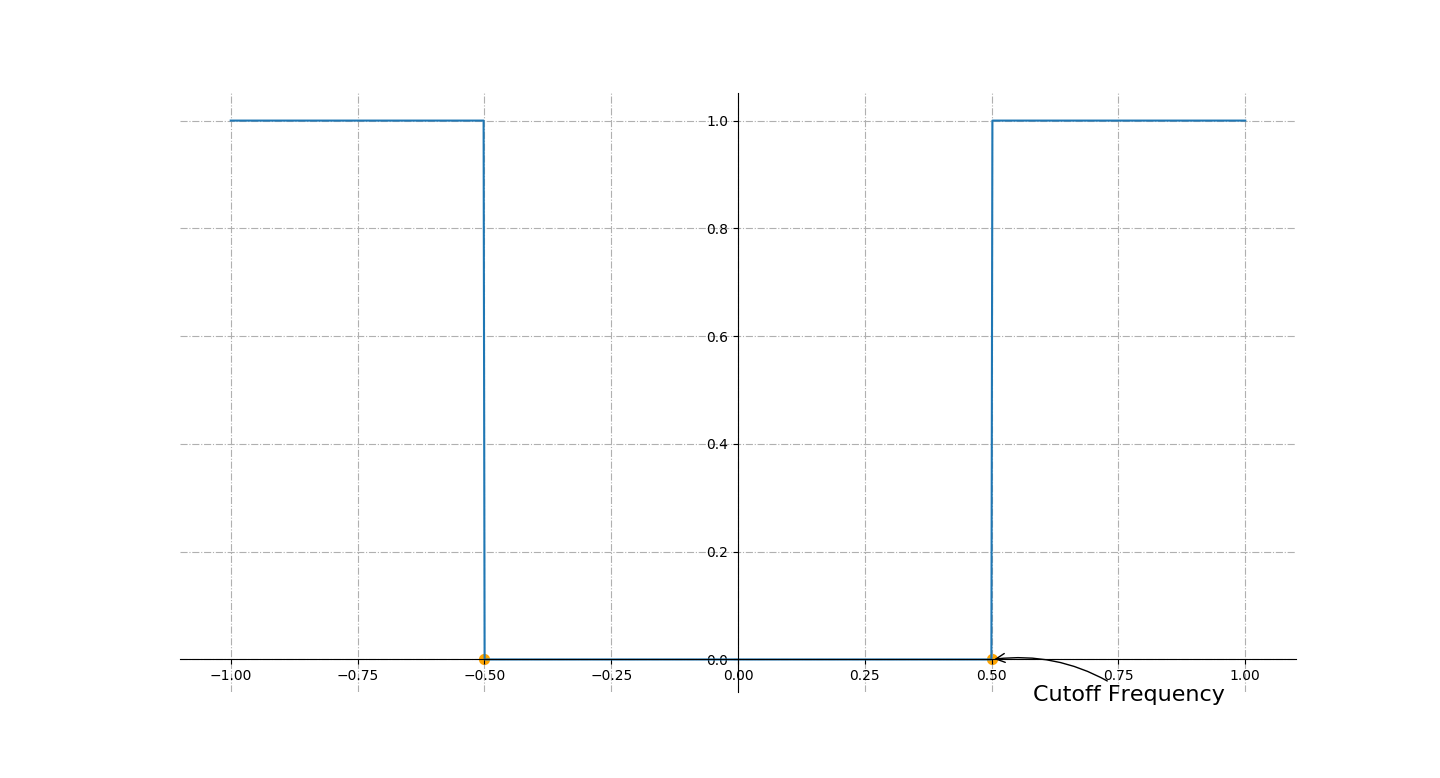
\includegraphics[width=0.4\textwidth]{assets/Figure_6.png}
	\caption{高通滤波器(High Pass Filter)}:常用于边缘检测。
\end{figure}
\begin{figure}[H]
	\centering
	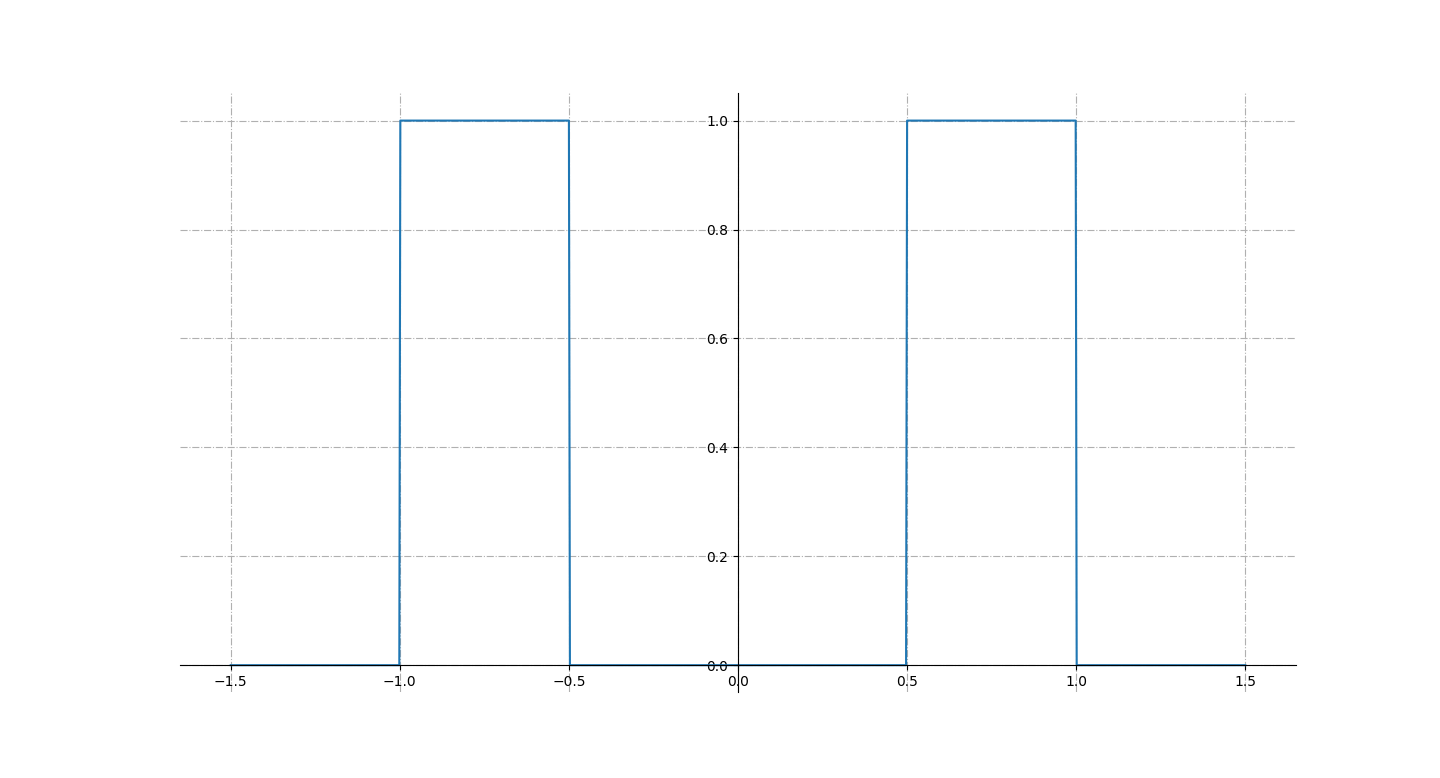
\includegraphics[width=0.4\textwidth]{assets/Figure_7.png}
	\caption{带通滤波器(Band Pass Filter)}
\end{figure}
%TODO:热方程
\section{Fourier Transform的导数定理}
\subsection{$\mathcal{F}f'(s)=2\cdot \pi\cdot i\cdot s\cdot \mathcal{F}f(s)$}
对原函数进行微分后,它的Fourier Transform等于其原函数的Fourier Transform乘以$2\cdot \pi\cdot i\cdot s$。

\begin{align*}
	f(t)                          & =\int_{-\infty}^{\infty}\ \mathcal{F}f(s)\cdot e^{2\cdot \pi\cdot i\cdot s\cdot t}\ ds                                 \\
	\frac{\partial f}{\partial t} & =\int_{-\infty}^{\infty}\ \mathcal{F}f(s)\cdot(2\cdot \pi\cdot i\cdot s\cdot e^{2\cdot \pi\cdot i\cdot s\cdot t})\ ds  \\
	                              & =\int_{-\infty}^{\infty}\ [2\cdot \pi\cdot i\cdot s\cdot \mathcal{F}f(s)]\cdot e^{2\cdot \pi\cdot i\cdot s\cdot t}\ ds
\end{align*}
推广开来有:
$$
	\mathcal{F}f^{(n)}(s)=(2\cdot \pi\cdot i\cdot s)^n\cdot \mathcal{F}f(s)
$$
\subsection{$(f*g)'=f'*g$}
\begin{align*}
	  & \mathcal{F}(f*g)'                                              \\
	= & (2\cdot \pi\cdot i\cdot s)\cdot \mathcal{F}(f*g)               \\
	= & (2\cdot \pi\cdot i\cdot s)\cdot \mathcal{F}f\cdot \mathcal{F}g \\
	= & \mathcal{F}f'\cdot \mathcal{F}g                                \\
	= & f'*g
\end{align*}
\begin{quote}
	Conv. comes into the solution of differential equations because often in solving differential equations if you take the Fourier Transform, differentiation becomes multiplication. And multiplication in the frequency domain becomes conv. in the time domain on taking Inverse Fourier Transform.
\end{quote}
$$
	Differentiation\stackrel{FT}\longrightarrow Multiplication\stackrel{IFT}\longrightarrow Conv.
$$
\section{正态分布}
\subsection{正态分布与标准分布}
若随机变量$X$服从一个位置参数为$\mu$,尺度参数为$\sigma$的正态分布,则其概率密度函数为:
$$
	f(x)=\frac{1}{\sigma\sqrt{2\cdot \pi}}\cdot e^{-\frac{(x-\mu)^2}{2\cdot \sigma^2}}
$$

正态分布的数学期望等于其位置参数$\mu$,其标准差等于尺度参数$\sigma$。
\subsection{归一化的高斯函数$f(t)=e^{-\pi\cdot t^2}$}
\subsubsection{对$f(t)=e^{-\pi\cdot t^2}$求$[0,1]$上的积分}
由于高斯函数的变量$t$在幂的位置上,而且是二次方,因此无法用$dt$对其进行积分计算,下面使用极座标法对其进行积分:
\begin{align*}
	  & (\int_{-\infty}^{\infty}\ e^{-\pi\cdot t^2}\ dt)^2                                        \\
	= & \int_{-\infty}^{\infty}\ e^{-\pi\cdot x^2}\ dx\cdot e^{-\pi\cdot y^2}\ dy                 \\
	= & \iint_{-\infty}^{\infty}\ e^{-\pi\cdot (x^2+y^2)}\ dx\ dy                                 \\
	= & \int_0^{2\cdot \pi} \int_0^{\infty}\ e^{-\pi\cdot r^2}\cdot r\ dr\ d\theta                \\
	= & 2\cdot \pi \int_0^{\infty}\ e^{-\pi\cdot r^2}\cdot r\ dr                                  \\
	= & 2\cdot \pi \int_0^{\infty}\ e^{-\pi\cdot r^2}\ d(\frac{1}{2}\cdot r^2)                    \\
	= & \frac{2\cdot \pi}{\pi}\cdot\frac{1}{2}\int_0^{\infty}\ e^{-\pi\cdot r^2}\ d(\pi\cdot r^2) \\
	= & \int_0^{\infty}\ e^{-s}\ ds=1
\end{align*}

\subsubsection{对$f(t)=e^{-\pi\cdot t^2}$求Fourier Transform}
$$
	\mathcal{F}f(s)=\int_{-\infty}^{\infty}\ e^{-2\cdot \pi\cdot i\cdot s\cdot t}\cdot e^{-\pi\cdot t^2}\ dt
$$
这是一个非常难以积分的项,我们需要采用其他巧妙的方法,微分:
\begin{align*}
	  & (\mathcal{F}f)'(s)                                                                                                      \\
	= & \int_{-\infty}^{\infty}\ \frac{d(e^{-2\cdot \pi\cdot i\cdot s\cdot t})}{ds}\cdot e^{-\pi\cdot t^2}\cdot dt              \\
	= & \int_{-\infty}^{\infty}\ -2\cdot\pi\cdot i\cdot t\cdot e^{-2\cdot \pi\cdot i\cdot s\cdot t}\cdot e^{-\pi\cdot t^2}\ dt  \\
	= & i\cdot \int_{-\infty}^{\infty}\ e^{-2\cdot \pi\cdot i\cdot s\cdot t}\cdot(-2\cdot\pi\cdot t\cdot e^{-\pi\cdot t^2})\ dt \\
	= & -2\cdot\pi\cdot s \int_{-\infty}^{\infty}\ e^{-2\cdot \pi\cdot i\cdot s\cdot t}\cdot e^{-2\cdot\pi\cdot t^2}\ dt        \\
	= & -2\cdot\pi\cdot s\cdot \mathcal{F}f(s)
\end{align*}

求解微分方程得:
\begin{align*}
	  & \mathcal{F}f(s)                                                       \\
	= & \mathcal{F}f(0)\cdot e^{-\pi\cdot s^2}                                \\
	= & \int_{-\infty}^{\infty}\ e^{-\pi\cdot t^2}\ dt\cdot e^{-\pi\cdot s^2} \\
	= & e^{-\pi\cdot s^2}
\end{align*}

也就是说归化为$1$的高斯函数的Fourier Transform还是归化为$1$的高斯函数:
\begin{equation}
	\mathcal{F}(e^{-\pi\cdot t^2})=e^{-\pi\cdot s^2}
\end{equation}
\begin{quote}
	傅立叶导数定理:
	\begin{align*}
		\begin{autobreak}
			\mathcal{F}f'(s)
			=2\cdot\pi\cdot i\cdot s\cdot \mathcal{F}f(s)
		\end{autobreak}
	\end{align*}

	注意区分!!!傅立叶导数定理是求$f$导数的Fourier Transform;上面是求$f$的Fourier Transform的导数。
\end{quote}

\section{分布与Convolution}
假设有两个独立的随机变量:$x_1$和$x2$,其密度函数分别为$p_1(x_1)$和$p_2(x_2)$。那么$x_1+x_2$的密度函数为$p_{12}(x_{12})$。

设有任意变量$t$,$\Prob(x_1+x_2\leq t)$意为坐标落在阴影部分的概率:
\begin{figure}[H]
	\centering
	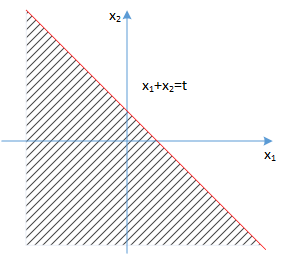
\includegraphics[width=0.4\textwidth]{assets/prob1.png}
	\caption{$x_1,x_2$平面}
\end{figure}
\begin{align*}
	  & \Prob(x_1+x_2\leq t)                                      \\
	= & \iint_{x_1+x_2\leq t}\ p_1(x_1)\cdot p_2(x_2)\ dx_1\ dx_2
\end{align*}

进行变量代换,令$u=x_1$,$v=x_1+x_2$,则:
$$
	\begin{cases}
		x_1 & =u   \\
		x_2 & =v-u \\
		t   & =v
	\end{cases}
$$
进行变量代换后,对应的新平面如下:
\begin{figure}[H]
	\centering
	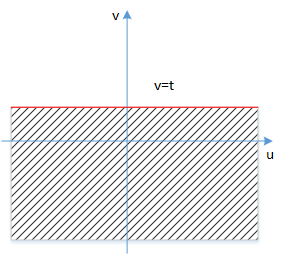
\includegraphics[width=0.4\textwidth]{assets/prob2.png}
	\caption{$u,v$平面}
\end{figure}
\begin{align*}
	  & \Prob(x_1+x_2\leq t)                                                        \\
	= & \Prob(v\leq t)                                                              \\
	= & \int_{-\infty}^{\infty}\ \int_{-\infty}^{t}\ p_1(u)\cdot p_2(v-u)\ du\ dv   \\
	= & \int_{-\infty}^{t}\ (\int_{-\infty}^{\infty}\ p_1(u)\cdot p_2(v-u)\ du)\ dv \\
	= & \int_{-\infty}^{t}\ (p_1*p_2)\ dv
\end{align*}

因此$p_1*p_2$可以作为$x_1+x_2$的密度函数。推广开来就是,独立随机变量的和的密度函数为他们各自密度函数的Convolution:
\begin{equation}
	p(x_1+x_2+\cdots+x_n)=p_1*p_2*\cdots *p_n
\end{equation}

\section{Fourier Transform与中心极限定理}
\subsection{中心极限定理}
在适当的条件下,大量相互独立随机变量的均值经适当标准化后依分布收敛于正态分布。
\subsubsection{Fourier Transform中}
%TODO:Fourier Transform中的复指形式的高斯分布和CLT中的高斯分布是什么关系??
在Fourier Transform中我们使用:
$$
	f(t)=e^{-\pi\cdot t^2}
$$
作为标准高斯分布,因为它的Fourier Transform和Inverse Fourier Transform都是$e^{-\pi\cdot t^2}$。
\subsubsection{CLT中}
标准正态分布的密度函数是:
$$
	p(x)=\frac{1}{\sqrt{2\cdot\pi}}\cdot e^{-\frac{x^2}{2}}
$$

采用这个式子作为标准正态分布的原因是它的均值(期望值)是$0$,它的标准差与方差为$1$。

\subsection{Convolution对函数的作用概览}
Several times we've met the idea that convolution is a smoothing
operation. Let me begin with somegraphical examples of this,
convolving a discontinuous or rough function repeatedly with itself.
For homework you computed, by hand, the convolution of the rectangle
function $\Pi$ with itself a few times.
\begin{figure}[H]
	\centering
	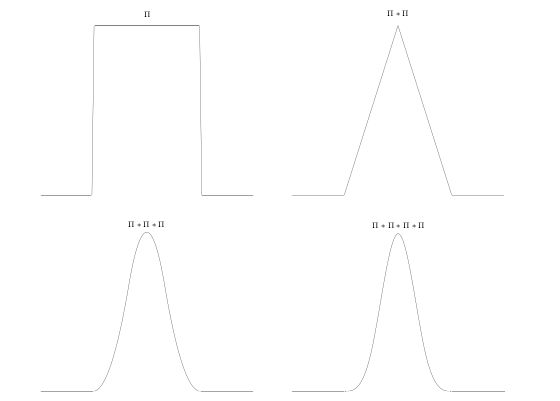
\includegraphics[scale=0.4]{assets/PI.jpg}
	\caption{$\pi$函数做Fourier Transform}
\end{figure}
Not only are the convolutions becoming smoother, but the
unmistakable shape of a Gaussian is emerging.Is this a coincidence,
based on the particularly simple nature of the function $\Pi$, or
is something more going on? Here is a plot of, literally, a random
function $f(x)$ --- the values $f(x)$ are just randomly chosen
numbers between 0 and 1.

\subsection{中心极限定理的推导过程}
\subsubsection{初始条件}
设有$n$个独立同分布的随机变量:$x_1,x_2,\cdots,x_n$,他们满足以下条件:
\begin{enumerate}
	\def\labelenumi{\arabic{enumi}.}
	\item
	      均值为$0$;
	\item
	      标准差为$1$。
\end{enumerate}
用$s_n$表示这$n$个随机变量的和,则$s_n$的密度函数为:
$$
	p^{*n}=\underbrace{p*p*\cdots *p}_{\text{n个p}}
$$

$S_n$的均值为$0$,标准差为$\sqrt{n}$,因此我们需要对它进行标准化(这里没咋太看懂),标准化后的密度函数为:
$$
	p_{normal}(x)=\sqrt{n}\cdot p^{*n}(\sqrt{n}\cdot x)
$$
\subsubsection{解答}
\begin{align*}
	        & \mathcal{F}p_{normal}(x)                                                                                                                                                     \\
	=       & \mathcal{F}(\sqrt{n}\cdot p^{*n})(\sqrt{n}\cdot x)                                                                                                                           \\
	=       & \sqrt{n}\cdot\frac{1}{\sqrt{n}}\cdot [\mathcal{F}(p^{*n})](\frac{s}{\sqrt{n}})                                                                                               \\
	=       & [\mathcal{F}(p^{*n})](\frac{s}{\sqrt{n}})                                                                                                                                    \\
	=       & (\mathcal{F}p)^n(\frac{s}{\sqrt{n}})                                                                                                                                         \\
	=       & [\int_{-\infty}^{\infty}\ e^{-2\cdot \pi\cdot i\cdot \frac{s}{\sqrt{n}}\cdot x}\cdot p(x)\ dx]^n                                                                             \\
	=       & [\int_{-\infty}^{\infty}\ [1-\frac{2\cdot \pi\cdot i\cdot s\cdot x}{\sqrt{n}}+\frac{1}{2}\cdot (\frac{2\cdot \pi\cdot i\cdot s\cdot x}{\sqrt{n}})^2+\cdots]\cdot p(x)\ dx]^n \\
	=       & [\int_{-\infty}^{\infty}\ p(x)\ dx-\frac{2\cdot \pi\cdot i\cdot s}{\sqrt{n}}\cdot \int_{-\infty}^{\infty}\ x\cdot p(x)\ dx                                                   \\
	-       & \frac{1}{2}\cdot (\frac{2\cdot \pi\cdot i\cdot s}{\sqrt{n}})^2\cdot \int_{-\infty}^{\infty}\ x^2\cdot p(x)\ dx+\cdots]^n                                                     \\
	=       & (1-0-\frac{2\cdot\pi^2\cdot s^2}{n}+\cdots)^n                                                                                                                                \\
	\approx & (1-\frac{2\cdot \pi^2\cdot s^2}{n})^n
\end{align*}

当$n\rightarrow\infty$时:
$$
	\lim\limits_{n\rightarrow\infty}(1-\frac{2\cdot \pi^2\cdot s^2}{n})^n\approx e^{-2\cdot\pi^2\cdot s^2}
$$

即:
$$
	\mathcal{F}(\sqrt{n}\cdot p^{*n})(\sqrt{n}\cdot x)=e^{-2\cdot\pi^2\cdot s^2}
$$
用Inverse Fourier Transform求出:
\begin{equation}
	p_{normal}=\mathcal{F}^{-1}(e^{-2\cdot\pi^2\cdot s^2})=\frac{1}{\sqrt{2\cdot \pi}}\cdot e^{-\frac{x^2}{2}}
\end{equation}
\chapter{广义傅立叶变换}
\section{传统傅立叶变换所存在的问题}
\subsection{传统傅立叶变换所存在的问题}
\begin{enumerate}
	\item 傅立叶变换基于积分的收敛;
	\item Inverse 傅立叶变换必须可行,否则尽管傅立叶变换被执行了也毫无意义。
\end{enumerate}
\subsection{问题例子}
\subsubsection{例子1}
令$f(t)=\Pi(t)$
\begin{enumerate}
	\item 傅立叶变换公式法计算
	      \begin{align*}
		      \mathcal{F}\Pi        & =\sinc                                  \\
		      \mathcal{F}^{-1}\sinc & =\mathcal{F}^{-1}\mathcal{F}\Pi=\pi     \\
		      \mathcal{F}\sinc      & =\mathcal{F}\mathcal{F}\Pi=\Pi^{-1}=\Pi
	      \end{align*}
	\item 积分方法计算
	      \begin{align*}
		      \mathcal{F}\Pi        & =\int_{-\infty}^{\infty}\ e^{-2\cdot \pi\cdot i\cdot s\cdot t}\ ds                                           \\
		      \mathcal{F}^{-1}\sinc & =\int_{-\infty}^{\infty}\ e^{2\cdot \pi\cdot i\cdot s\cdot t}\cdot \frac{\sinc (\pi\cdot s)}{\pi\cdot s}\ ds \\
		      \mathcal{F}\sinc      & =\int_{-\infty}^{\infty}\ e^{-2\cdot \pi\cdot i\cdot s\cdot t}\cdot \frac{\sin (\pi\cdot s)}{\pi\cdot s}\ ds
	      \end{align*}
\end{enumerate}

在傅立叶变换公式法计算中,我们能很轻松地运用傅里叶的逆变换、对偶等定理得到结果。

但是在实际应用中我们对信号进行傅里叶转换并处理后,通常需要用积分方法进行计算后去获得原始的信号,而积分方法的第二三个式子的积分求法是非常困难的。

另外,在计算的时候还必须面对一些函数的收敛性问题——由于$\Pi$函数是跳跃的,最终积分运算得到的$\Pi$会在跳变点$\pm \frac{1}{2}$处取值为$\frac{1}{2}\cdot (0+1)$。
\subsubsection{例子2}
\begin{align*}
	 & f(t)  =1                                                                                                       \\
	 & \mathcal{F}f(t)=\int_{-\infty}^{\infty}\ e^{-2\cdot \pi\cdot i\cdot s\cdot t}\ dt                              \\
	 & f(t) =\sin(2\cdot\pi\cdot t)                                                                                   \\
	 & \mathcal{F}f(t)  =\int_{-\infty}^{\infty}\ e^{-2\cdot \pi\cdot i\cdot s\cdot t}\cdot\sin(2\cdot\pi\cdot t)\ dt \\
	 & f(t)=\cos(2\cdot\pi\cdot t)                                                                                    \\
	 & \mathcal{F}f(t)=\int_{-\infty}^{\infty}\ e^{-2\cdot \pi\cdot i\cdot s\cdot t}\cdot \cos(2\cdot\pi\cdot t)\ dt
\end{align*}

对于这些不收敛的函数的积分是无意义的。
\section{Schwartz Space}
定义最适合傅立叶变换的函数$\mathcal  {S}$,我们称之为速降函数。
\subsection{定义}
$f(x)$是无限可微的,对于任何$m,n\geq 0$,都有:
$$
	\lim\limits_{t\rightarrow\pm\infty}|t|^n\cdot |\frac{\partial^m}{(\partial t)^m}f(t)|=0
$$

这个式子表明:$f(t)$的任意阶导数趋于$0$的速度都比$t$的任意次方上升的速度快。
\subsection{性质}
因为速降函数有如下性质,所以速降函数是傅立叶变换的最佳函数:
\begin{enumerate}
	\item 如果$f(t)\in \mathcal  {S}$,那么$\mathcal{F}f(t)\in \mathcal  {S}$;
	\item 如果$f(t)\in \mathcal  {S}$,那么$\mathcal{F}^{-1}f(t)\in \mathcal  {S}$;
	\item 正负傅立叶变换:
	      \begin{align*}
		      \mathcal{F}\mathcal{F}^{-1}f=f \\
		      \mathcal{F}^{-1}\mathcal{F}f=f
	      \end{align*}
\end{enumerate}

$\Pi\notin \mathcal  {S}$,因为不连续;$\Lambda\notin \mathcal  {S}$,因为不可微;$\mathbb{R},\cos,\sin \notin \mathcal  {S}$,因为不速降。

\section{Parserval等式}
\begin{quote}
	该等式在傅立叶变换中被称为Railey's Identity,在傅立叶级数中被称为Parserval's Identity。
\end{quote}
\subsection{定义}
设有$f(x),g(x)\in \mathcal  {S}$,则:
\begin{equation}
	\int_{-\infty}^{\infty}\ |\mathcal{F}f(s)|^2\ ds=\int_{-\infty}^{\infty}\ |f(x)|^2\ dx
\end{equation}
\begin{enumerate}
	\item 左边:$\mathcal  {S}$函数進行傅立叶变换仍爲$\mathcal  {S}$函数,因此左边收敛;
	\item 右边:对于$\mathcal  {S}$函数不用担心积分收敛问题,因为它们衰减很快,积分必然收敛。
\end{enumerate}
\subsection{注解}
\begin{enumerate}
	\def\labelenumi{\arabic{enumi}.}
	\item
	      信号在时域与频域的能量相等;
	\item
	      设有$f(t),g(t)\in \mathcal  {S}$,则:

	      $$
		      \int_{-\infty}^{\infty}\ \mathcal{F}f(s)\cdot \mathcal{F}\overline{g}(s)\ ds=\int_{-\infty}^{\infty}\ f(s)\cdot \overline{g}(x)\ dx
	      $$
\end{enumerate}
\subsection{证明}
因为:
$$
	g(s)=\int_{-\infty}^{\infty}\ e^{2\cdot \pi\cdot i\cdot s\cdot x}\cdot \mathcal{F}g(s)\ ds
$$

所以:
$$
	\overline{g}(s)=\int_{-\infty}^{\infty}\ e^{-2\cdot \pi\cdot i\cdot s\cdot x}\cdot \mathcal{F}\overline{g}(s)\ ds
$$

所以:
\begin{align*}
	  & \int_{-\infty}^{\infty}\ f(x)\cdot \overline{g}(x)\ dx                                                                                     \\
	= & \int_{-\infty}^{\infty}\ f(x)\cdot(\int_{-\infty}^{\infty}\ e^{-2\cdot \pi\cdot i\cdot s\cdot x}\cdot \mathcal{F}\overline{g}(s)\ ds)\ dx  \\
	= & \int_{-\infty}^{\infty}\ (\int_{-\infty}^{\infty}\ f(x)\cdot e^{-2\cdot \pi\cdot i\cdot s\cdot x}\ dt)\cdot \mathcal{F}\overline{g}(s)\ ds \\
	= & \int_{-\infty}^{\infty}\ \mathcal{F}f(s)\cdot\mathcal{F}\overline{g}(s)\ ds
\end{align*}

同理,由于$|e^{2\cdot \pi\cdot i\cdot s\cdot x}|=1$,因此:

\[\int_{-\infty}^{\infty}\ |\mathcal{F}f(s)|^2\ ds=\int_{-\infty}^{\infty}\ |f(x)|^2\ dx\]

\section{脉冲函数$\delta$}
$\delta$ is supposed to represent a function which is concentrated at a point.
\subsection{如何得到$\delta$}
我们利用$\Pi$函数的宽度不断缩小来逼近$\Pi$。
\begin{figure}[H]
	\centering
	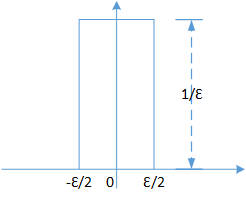
\includegraphics[width=0.4\textwidth]{assets/delta.png}
	\caption{$\delta=\lim\limits_{\epsilon\rightarrow 0}\ \frac{1}{\epsilon}\cdot \Pi_\epsilon(x)$}
\end{figure}
\subsection{脉冲函数的性质}
\begin{enumerate}
	\item $\delta$函数的积分为$1$:
	      $$
		      \int_{-\infty}^{\infty}\ \frac{1}{\epsilon}\cdot \Pi_\epsilon(x)\ dx=\frac{1}{\epsilon}\cdot \int_{-\frac{\epsilon}{2}}^{\frac{\epsilon}{2}}\ 1\ dx=1
	      $$
	\item 如果单单观察$\delta$函数是没有意义的,但是如果$\delta$函数乘上某个函数再积分,就能得到函数在$0$点的值:
	      \begin{align*}
		        & \int_{-\infty}^{\infty}\ \frac{1}{\epsilon}\cdot \Pi_\epsilon(x)\cdot \phi(x)\ dx                                                           \\
		      = & \frac{1}{\epsilon}\cdot \int_{-\frac{\epsilon}{2}}^{\frac{\epsilon}{2}}\ \phi(x)\ dx                                                        \\
		      = & \frac{1}{\epsilon}\cdot \int_{-\frac{\epsilon}{2}}^{\frac{\epsilon}{2}}\ [\phi(0)+\phi'(0)\cdot x+\frac{1}{2}\phi''(0)\cdot x^2+\cdots]\ dx \\
		      = & \phi(0)+o(\epsilon)  = \phi(0)
	      \end{align*}
\end{enumerate}
\subsection{$\delta$的移位}
$$
	\int_{-\infty}^{\infty}\ \delta(a-y)\cdot f(y)\ dy=f(a)
$$
该式子表明了$\delta$从位置$a$处获得函数$f$的值$f(a)$f。我们前面讨论的是$x=0$的情况,在这里,我们定义了一个新的分布,我们记该分布为$\delta_a$。
\subsection{$\delta$的抽样特性}
证明利用到了分布的乘积性质。设有函数$f$:
\begin{align*}
	  & <f\cdot \delta,\phi>                                  \\
	= & <\delta,f\cdot \phi>                                  \\
	= & (f\cdot \phi)(0)   \quad (View\ f(0)\ as\ a\ number.) \\
	= & f(0)\cdot \phi(0)                                     \\
	= & <f(0)\delta,\phi>                                     \\
\end{align*}

因此:
\begin{equation}
	f\cdot \delta=f(0)\cdot \delta
\end{equation}

同理:
\begin{equation}
	f\cdot \delta_a=f(a)\cdot \delta_a
\end{equation}
\subsection{$\delta$的平移特性}
该式子证明利用到了分布的卷积性质。

\subsection{函数$f$与$\delta_a$进行卷积}
\begin{align*}
	  & <f*\delta_a,\phi>                                              \\
	= & <f(x),<\delta_a(y),\phi(x+y)>>                                 \\
	= & <f(x),\phi(x+a)>                                               \\
	= & \int_{-\infty}^{\infty}\ f(u-a)\cdot \phi(u)\ du \quad (u=x+a) \\
	= & <f(u-a),\phi>
\end{align*}

$f$与$\delta_a$进行卷积会导致$f$右移$a$个单位:
\begin{equation}
	f(x)*\delta_a=f(x-a)
\end{equation}

同理可以推导出:
\begin{equation}
	\delta_a*\delta_b=\delta_{a+b}
\end{equation}
\subsection{$\delta$的缩放特性}
该式子证明利用到了分布的卷积性质。

$\delta(x)$是集中于一点的脉冲函数,因此按照我们主观的印象来说,无论怎么在$x$轴对其缩放,都还是原来的脉冲函数,但是事实并不是这样的,我们可以观察下面的推理过程。

当$a>0$时:
\begin{align*}
	  & <\delta(a\cdot x),\phi(x)>                                                                  \\
	= & \int_{-\infty}^{\infty}\ \delta(a\cdot x)\cdot \phi(x)\ dx                                  \\
	= & \int_{-\infty}^{\infty}\ \delta(u)\cdot \phi(\frac{u}{a})\ d(\frac{u}{a})\quad (u=a\cdot x) \\
	= & \frac{1}{a}\cdot \int_{-\infty}^{\infty}\ \delta(u)\cdot \phi(\frac{u}{a})\ du              \\
	= & \frac{1}{a}\cdot<\delta(u),\phi(\frac{u}{a})>                                               \\
	= & \frac{1}{a}\cdot \phi(0)                                                                    \\
	= & <\frac{1}{a}\cdot \delta(x),\phi(x)>
\end{align*}

当$a<0$时:
\begin{align*}
	  & <\delta(a\cdot x),\phi(x)>                                                                  \\
	= & \int_{-\infty}^{\infty}\ \delta(a\cdot x)\cdot \phi(x)\ dx                                  \\
	= & \int_{-\infty}^{\infty}\ \delta(u)\cdot \phi(\frac{u}{a})\ d(\frac{u}{a})\quad (u=a\cdot x) \\
	= & \frac{1}{a}\cdot \int_{\infty}^{-\infty}\ \delta(u)\cdot \phi(\frac{u}{a})\ du              \\
	= & -\frac{1}{a}\cdot<\delta(u),\phi(\frac{u}{a})>                                              \\
	= & -\frac{1}{a}\cdot \phi(0)                                                                   \\
	= & <-\frac{1}{a}\cdot \delta(x),\phi(x)>
\end{align*}

因此:
\begin{equation}
	\delta(a\cdot x)=\frac{1}{|a|}\cdot \delta
\end{equation}
\section{分布}
这里的分布不同于概率上的分布,它是广义函数(generalized function)的另一种说法。
\subsection{测试函数$\phi$}
对于当前研究是最优函数。对于傅立叶变换来说,最优函数就是速降函数。
\subsection{广义函数Generalized Function}
跟这些测试函数相关的,我们称之为广义函数或者分布。

Associated with these test functions is a class of what are called generalized functions of distributions.

一个分布$T$是一个作用于测试函数的线性算子,它作用于测试函数后会产生一个数值,即$T(\phi)$会得到一个数。

A distribution is a linear operation on the test functions that produces a number.

$T$是$\phi$的线性泛函:

The distribution $T$ is a linear functional on test functions.

\begin{align*}
	T(\phi_1+\phi_2)    & =T(\phi_1)+T(\phi_2) \\
	T(\alpha\cdot \phi) & =\alpha\cdot T(\phi)
\end{align*}
\subsection{匹配}
分布作用于$\phi$,我们常称之为匹配,记为$<T,\phi>$:
\begin{equation}
	<T,\phi> = \int_{-\infty}^{\infty}\ T(x)\cdot \phi(x)\ dx
\end{equation}

可以把$\phi$想象成一些物理信息的分布,$T$是一种测量它的方法。使用测量方法去测量一个信息,你将得到一个数。

并非所有函数都会在匹配后积分收敛,但是大多数的函数甚至特别奇异的函数都能使积分收敛,匹配成功。

\subsection{分布的性质}
\begin{enumerate}
	\item 线性
	\item 如果$\phi_n$是一个函数序列收敛于$\phi$,那么如果用$T$作用于$\phi_n$,它也将收敛于$T(\phi)$。
\end{enumerate}



\section{分布傅立叶变换}
\subsection{缓增函数}
在傅立叶变换中,测试函数$\phi$为速降函数。与之对应的分布$T$通常被称为缓增函数(Tempered Distributions):
$$
	<T,\phi>=\int_{-\infty}^{\infty}\ T(x)\cdot \phi(x)\ dx
$$
\subsection{缓增函数的傅立叶变换}
\subsubsection{定义}
定义缓增分布$T$的傅立叶变换为$\mathcal{F}T$,$\mathcal{F}T$作用于速降函数$\phi$就相当于$T$作用于速降函数的傅立叶变换 $\mathcal{F}\phi$:
\begin{equation}
	<\mathcal{F}T,\phi>=<T,\mathcal{F}\phi>
\end{equation}
同理可得,分布的Inverse 傅立叶变换为:
\begin{equation}
	<\mathcal{F}^{-1}T,\phi>=<T,\mathcal{F}^{-1}\phi>
\end{equation}
\subsubsection{证明}
\begin{align*}
	  & <\mathcal{F}T,\phi>                                                                                                     \\
	= & \int_{-\infty}^{\infty}\ \mathcal{F}T(x)\cdot \phi(x)\ dx                                                               \\
	= & \int_{-\infty}^{\infty}\ (\int_{-\infty}^{\infty}\ e^{-2\cdot \pi\cdot i\cdot x\cdot y}\cdot T(y)\ dy)\cdot \phi(x)\ dx \\
	= & \int_{-\infty}^{\infty}\ (\int_{-\infty}^{\infty}\ e^{-2\cdot \pi\cdot i\cdot x\cdot y}\cdot \phi(x)\ dx)\cdot T(y)\ dy \\
	= & \int_{-\infty}^{\infty}\ \mathcal{F}\phi(y)\cdot T(y)\ dy                                                               \\
	= & <T,\mathcal{F}\phi>
\end{align*}

因为$\phi\in \mathcal  {S}$,所以$\mathcal{F}\phi\in \mathcal  {S}$,因此$<T,\mathcal{F}\phi>$是有意义的。至于$<\mathcal{F}T,\phi>$有没有意义,nobody cares。
\subsection{分布傅立叶变换的例子}
\subsubsection{$\mathcal{F}\sigma$}
\begin{align*}
	  & <\mathcal{F}\sigma,\phi>  =  <\sigma,\mathcal{F}\phi>                          \\
	= & \mathcal{F}\phi(0)                                                             \\
	= & \int_{-\infty}^{\infty}\ e^{-2\cdot \pi\cdot i\cdot 0\cdot x}\cdot \phi(x)\ dx \\
	= & \int_{-\infty}^{\infty}\ 1\cdot \phi(x)\ dx                                    \\
	= & <1,\phi>
\end{align*}

因此:
\begin{equation}
	\mathcal{F}\sigma=1
\end{equation}
\begin{figure}[H]
	\centering
	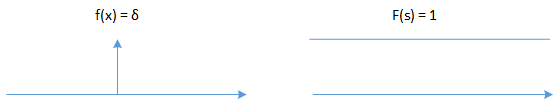
\includegraphics[width=0.4\textwidth]{assets/fdelta.png}
\end{figure}
在$\sigma$的定义中,我们知道$\sigma$无限集中于$0$点,我们通过$\Pi$函数的极限形式来逼近它。而它的傅里叶变换为$1$,这是均匀散开的。还记得我们曾经在讨论傅里叶缩放的时候讲过——时域的集中会导致频域的分散,这就是一个极端的例子。
\subsubsection{$\mathcal{F}\sigma_a$}
\begin{align*}
	  & <\mathcal{F}\sigma_a,\phi>  =  <\sigma_a,\mathcal{F}\phi>                      \\
	= & \mathcal{F}\phi(a)                                                             \\
	= & \int_{-\infty}^{\infty}\ e^{-2\cdot \pi\cdot i\cdot a\cdot x}\cdot \phi(x)\ dx \\
	= & <e^{-2\cdot \pi\cdot i\cdot a\cdot x},\phi>
\end{align*}

因此:
\begin{equation}
	\mathcal{F}\sigma_a=e^{-2\cdot \pi\cdot i\cdot a\cdot x}
\end{equation}

\subsubsection{$\mathcal{F}e^{2\cdot \pi\cdot i\cdot a\cdot x}$}
\begin{align*}
	  & <\mathcal{F}e^{2\cdot \pi\cdot i\cdot a\cdot x},\phi>  =  <e^{2\cdot \pi\cdot i\cdot a\cdot x},\mathcal{F}\phi> \\
	= & \int_{-\infty}^{\infty}\ e^{2\cdot \pi\cdot i\cdot a\cdot x}\cdot \mathcal{F}\phi(x)\ dx                        \\
	= & \mathcal{F}^{-1}\mathcal{F}\phi(a)                                                                              \\
	= & \phi(a)= <\sigma_a,\phi>
\end{align*}

因此:
\begin{equation}
	\mathcal{F}e^{2\cdot \pi\cdot i\cdot a\cdot x}=\sigma_a
\end{equation}
\begin{figure}[H]
	\centering
	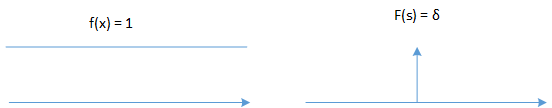
\includegraphics[width=0.4\textwidth]{assets/fe.png}
\end{figure}
当$a=0$时,$e^{2\cdot \pi\cdot i\cdot a\cdot x}=1$,则$\mathcal{F}1=\sigma$。$f(x)=1$的傅里叶变换为$\sigma$,这是一个时域分散导致频域集中的极端例子。
\subsubsection{$\mathcal{F}\cos(2\cdot\pi\cdot a\cdot x)$}
\begin{align*}
	  & \mathcal{F}\cos(2\cdot\pi\cdot a\cdot x)                                                                         \\
	= & \mathcal{F}[\frac{1}{2}\cdot(e^{2\cdot \pi\cdot i\cdot a\cdot x}+e^{-2\cdot \pi\cdot i\cdot a\cdot x})]          \\
	= & \frac{1}{2}\cdot(\mathcal{F}e^{2\cdot \pi\cdot i\cdot a\cdot x}+\mathcal{F}e^{-2\cdot \pi\cdot i\cdot a\cdot x}) \\
	= & \frac{1}{2}\cdot (\sigma_a+\sigma_{-a})
\end{align*}
\begin{figure}[H]
	\centering
	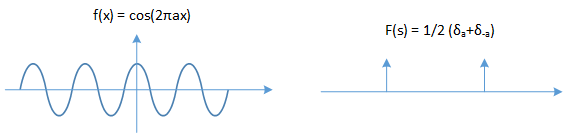
\includegraphics[width=0.4\textwidth]{assets/fcos.png}
\end{figure}
\subsubsection{$\mathcal{F}\sin(2\cdot\pi\cdot a\cdot x)$}
\begin{align*}
	  & \mathcal{F}\sin(2\cdot\pi\cdot a\cdot x)                                                                                \\
	= & \mathcal{F}[\frac{1}{2\cdot i}\cdot(e^{2\cdot \pi\cdot i\cdot a\cdot x}-e^{-2\cdot \pi\cdot i\cdot a\cdot x})]          \\
	= & \frac{1}{2\cdot i}\cdot(\mathcal{F}e^{2\cdot \pi\cdot i\cdot a\cdot x}-\mathcal{F}e^{-2\cdot \pi\cdot i\cdot a\cdot x}) \\
	= & \frac{1}{2\cdot i}\cdot (\sigma_a-\sigma_{-a})
\end{align*}
\begin{figure}[H]
	\centering
	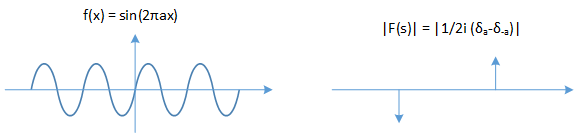
\includegraphics[width=0.4\textwidth]{assets/fsin.png}
\end{figure}
\section{分布与导数}
\subsection{相关定理}
\subsubsection{分布的导数}
\begin{align*}
	  & <T',\phi>                                                                                \\
	= & \int_{-\infty}^{\infty}\ T'(x)\cdot \phi(x)\ dx                                          \\
	= & \rsx{T(x)\cdot \phi(x)}_{-\infty}^\infty-\int_{-\infty}^{\infty}\ T(x)\cdot \phi'(x)\ dx \\
	= & 0-\int_{-\infty}^{\infty}\ T(x)\cdot \phi'(x)\ dx                                        \\
	= & -<T,\phi'>
\end{align*}

所以我们得到:
\begin{equation}
	<T',\phi>=-<T,\phi'>
\end{equation}

由速降函数可知,速降函数的任意阶导都比$x$的任意次幂衰减地都快,即速降函数的任意阶导都是速降函数。因此$\phi'\in \mathcal  {S}$,$<T,\phi'>$仍然成立。
\subsubsection{分布傅立叶变换的导数定理}
分布傅立叶变换的导数定理与傅立叶变换的导数定理类似,注意下面等式中的$s$与$t$:
\begin{equation}
	\mathcal{F}(T')=2\cdot\pi\cdot i\cdot s\cdot \mathcal{F}T
\end{equation}
\begin{equation}
	(\mathcal{F}T)'=\mathcal{F}(-2\cdot\pi\cdot i\cdot t\cdot T)
\end{equation}

\subsection{利用分布求导数的例子}
\subsubsection {单位跃阶函数(Unit Step function)}
\begin{figure}[H]
	\centering
	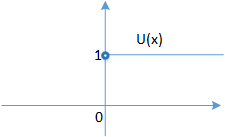
\includegraphics[width=0.4\textwidth]{assets/U_function.png}
	\caption{$\sin(2\cdot\pi\cdot t)+\sin(4\cdot\pi\cdot t)+\sin(8\cdot\pi\cdot t)$}
\end{figure}
\begin{align*}
	U(x)=
	\begin{cases}
		1 & x>0    \\
		0 & x\leq0
	\end{cases}
\end{align*}
下面开始求导:
\begin{align*}
	  & <U',\phi>=-<U(x),\phi'(x)>                                                  \\
	= & -\int_{-\infty}^{\infty}\ U(x)\cdot \phi'(x)\ dx                            \\
	= & -\int_{0}^{\infty}\ \phi'(x)\ dx                                            \\
	= & -\rsx{\phi(x)}_0^\infty                                                     \\
	= & -[0-\phi(0)]   \quad  (\because \lim\limits_{x\rightarrow\pm\inf}\phi(x)=0) \\
	= & \phi(0) = <\delta,\phi>
\end{align*}
因此:
\begin{equation}
	U'=\delta
\end{equation}

由于$U$在原点处有一个跃变,因此它在原点处导数无限大。
\subsubsection {有符号函数(Signum function)}
\begin{figure}[H]
	\centering
	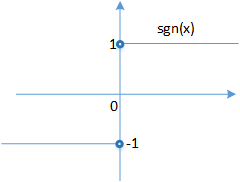
\includegraphics[width=0.4\textwidth]{assets/sgn_function.png}
	\caption{$\sin(2\cdot\pi\cdot t)+\sin(4\cdot\pi\cdot t)+\sin(8\cdot\pi\cdot t)$}
\end{figure}
\begin{align*}
	\sgn(x)=
	\begin{cases}
		1  & x>0 \\
		0  & x=0 \\
		-1 & x<0 \\
	\end{cases}
\end{align*}
下面开始求导:
\begin{align*}
	  & <\sgn',\phi>=<\sgn,\phi'>                                                          \\
	= & -\int_{-\infty}^{\infty}\ \sgn(x)\cdot \phi'(x)\ dx                                \\
	= & -[\int_{-\infty}^{0}\ -1\cdot \phi'(x)\ dx+\int_{0}^{\infty}\ 1\cdot \phi'(x)\ dx] \\
	= & \rsx{\phi(x)}_0^\infty=2\cdot \phi(0)=<2\cdot \sigma,\phi>
\end{align*}
因此:
\begin{equation}
	\sgn'=2\cdot \sigma
\end{equation}

下面求$\sgn$的导数:
\begin{align*}
	  & \mathcal{F}(\sgn)                                             \\
	= & \frac{\mathcal{F}(\sgn')}{2\cdot\pi\cdot i\cdot s}            \\
	= & \frac{2\cdot \delta}{2\cdot\pi\cdot i\cdot s}                 \\
	= & \frac{2}{2\cdot\pi\cdot i\cdot s}=\frac{1}{\pi\cdot i\cdot s} \\
\end{align*}

\subsection{利用导数求傅立叶变换}
\subsubsection {$\sgn$的傅立叶变换}
\begin{align*}
	  & \mathcal{F}(\sgn)                                             \\
	= & \frac{\mathcal{F}(\sgn')}{2\cdot\pi\cdot i\cdot s}            \\
	= & \frac{2\cdot \delta}{2\cdot\pi\cdot i\cdot s}                 \\
	= & \frac{2}{2\cdot\pi\cdot i\cdot s}=\frac{1}{\pi\cdot i\cdot s} \\
\end{align*}
\subsubsection {$U$的傅立叶变换}
\begin{align*}
	U            & =\frac{1}{2}\cdot(1+\sgn)                                                                  \\
	\mathcal{F}U & =\frac{1}{2}\cdot \mathcal{F}(1+\sgn)=\frac{1}{2}\cdot(\sigma+\frac{1}{\pi\cdot i\cdot s})
\end{align*}

在高通滤波器中会用到$U$(单位跃阶)这个信号,采用$U$的傅立叶变换将会加快处理过程。




\section{分布的乘积}
通常情况下被定义为函数与分布的乘积。
设有分布$T$,函数$f$:
\begin{align*}
	  & <T\cdot f,\phi>                                          \\
	= & \int_{-\infty}^{\infty}\ T(x)\cdot f(x)\cdot \phi(x)\ dx \\
	= & <T,f\cdot \phi>
\end{align*}
\section{分布与卷积}
\subsection{分布的卷积}
假设有函数$f$与速降函数$\psi$,他们的卷积为$f*\psi$:
\begin{align*}
	  & <\psi*f,\phi>                                                                                  \\
	= & \int_{-\infty}^{\infty}\ (\psi*f)(x)\cdot \phi(x)\ dx                                          \\
	= & \int_{-\infty}^{\infty}\ [\int_{-\infty}^{\infty}\ \psi(x-y)\cdot f(y)\ dy]\cdot \phi(x)\ dx   \\
	= & \int_{-\infty}^{\infty}\ [\int_{-\infty}^{\infty}\ \psi(x-y)\cdot \phi(x)\ dx]\cdot f(y)\ dy   \\
	= & \int_{-\infty}^{\infty}\ [\int_{-\infty}^{\infty}\ \psi^-(y-x)\cdot \phi(x)\ dx]\cdot f(y)\ dy \\
	= & \int_{-\infty}^{\infty}\ (\psi^-*\phi)(y)\cdot f(y)\ dy                                        \\
	= & <f,\psi^-*\phi>
\end{align*}

进一步推导:
\begin{align*}
	  & \psi^-*\phi                                                       \\
	= & \int_{-\infty}^{\infty}\ \psi(x-y)\cdot \phi(x)\ dx               \\
	= & \int_{-\infty}^{\infty}\ \psi(u)\cdot \phi(u+y)\ du \quad (u=x-y) \\
	= & <\psi(u),\phi(u+y)>
\end{align*}

把推导结果代入卷积的推导中,得:
$$
	<\psi*f,\phi>=<f(x),<\psi(y),\phi(x+y)>>
$$

推广到一般的分布中去,设有分布$S$和$T$:
\begin{equation}
	<S*T,\phi>=<S(x),<T(y),\phi(x+y)>>
\end{equation}

分布卷积成立的条件如下:

$<T(y),\phi(x+y)>$将产生一个变量为$x$的函数,只有当该函数为测试函数时,$S*T$才有意义。
\subsection{分布的卷积定理}
我们在分析传统傅立叶变换的卷积定理的时候,是结合卷积与傅立叶变换一起讨论的。在分布中,通常也会把卷积与傅立叶变换一起讨论。
\begin{align*}
	  & <\mathcal{F}(S*T),\phi>                     \\
	= & <S*T,\mathcal{F}\phi>                       \\
	= & <S,T^-*\mathcal{F}\phi>                     \\
	= & <S,\mathcal{F}\mathcal{F}T*\mathcal{F}\phi> \\
	= & <S,\mathcal{F}(\mathcal{F}T\cdot \phi)>     \\
	= & <\mathcal{F}S,\mathcal{F}T\cdot \phi>       \\
	= & <\mathcal{F}S\cdot \mathcal{F}T,\phi>
\end{align*}

因此:
\begin{equation}
	\mathcal{F}(S*T)=\mathcal{F}S\cdot \mathcal{F}T
\end{equation}
该定理成立的条件与卷积成立的条件一致,即$T^−$与速降函数进行卷积后仍然是速降函数。
\chapter{离散傅立叶变换}
\section{离散傅立叶变换}
欢迎从连续的、模拟的旧世界,来到离散的、数字的新世界!!!

$f(t)$为连续的信号,即$t$是一个连续变量:
\begin{enumerate}
	\item 找到一种合理的离散逼近$f(t)$的形式;
	\item 找到一种合理的离散的逼近$f(t)$的傅立叶变换 $\mathcal{F}f(s)$的形式;
	\item 找到一种从$f$的离散形式到傅立叶变换 $\mathcal{F}f$的离散形式的合理方法。
\end{enumerate}

下面的推导将建立在抽样定理的误用上:
\begin{enumerate}
	\item $f(t)$受限于$0\leq t\leq L$;
	\item $\mathcal{F}f(s)$受限于$0\leq s\leq 2\cdot B$
\end{enumerate}

为什么称之为误用基于两个原因:
\begin{enumerate}
	\item 我们知道频域上的带宽是$-B\leq s\leq B$这种形式,但是这里为了方便后面的推导,采用了上方的这种形式。
	\item 实际上这两个假设并不能同时成立,信号不可能同时在时域和频域上都受限。
\end{enumerate}

\subsection{$f(t)$的离散近似}
为了得到一个$f(t)$的离散近似,我们需要在以$\frac{1}{2\cdot B}$为间隔进行采样:
\begin{figure}[H]
	\centering
	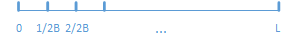
\includegraphics[width=0.4\textwidth]{assets/DFT1.png}
\end{figure}
设$f(t)$内共有$N$个采样点,即:$N\cdot \frac{1}{2\cdot B}=L$,则$N=2\cdot B\cdot N$。

令$t_0=0,t_1=\frac{1}{2\cdot B},\cdots,t_{N-1}=\frac{N-1}{2\cdot B}$。

对$f(t)$进行采样,得:
\begin{align*}
	  & f_{sample}(t)                                      \\
	= & f(t)\cdot \sum\limits_{k=0}^{N-1}\ \sigma(t-t_k)   \\
	= & \sum\limits_{k=0}^{N-1}\ f(t_k)\cdot \sigma(t-t_k)
\end{align*}

采样得到的项分离出$f(t)$的离散近似为:$f(t_0),f(t_1),\cdots,f(t_{N-1})$

但是采样后的$f$仍然是一个连续函数,我们可以对其进行傅立叶变换:
$$
	\mathcal{F}f_{sample}(s)=\sum\limits_{k=0}^{N-1}\ f(t_k)\cdot e^{-2\cdot \pi\cdot i\cdot s\cdot t_k}
$$
\begin{quote}
	就像泰勒级数可以在某一点展开一样,这里只是在$t=t_k$处展开。所以我们说采样后的$f$仍然是一个连续函数。
\end{quote}
\subsection{$\mathcal{F}f(s)$的离散近似}
为了离散化$\mathcal{F}f_{sample}(s)$,我们需要在频域进行采样。
\begin{figure}[H]
	\centering
	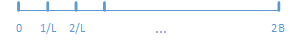
\includegraphics[width=0.4\textwidth]{assets/DFT2.png}
\end{figure}
关于采样,信号的采样频率是依据该信号在另一个域的性质决定的。
\begin{enumerate}
	\item 我们在时域采样时依据它在频域受限于$[0,2\cdot B]$;
	\item 而在频域采样是依据它在时域受限于$[0,L]$,即采样间隔为$\frac{1}{L}$。
\end{enumerate}


设$\mathcal{F}f(s)$上共有$M$个采样点,即:$M\cdot \frac{1}{L}=2\cdot B$,则:$M=2\cdot B\cdot L=N$。我们发现,时域与频域上的采样点数目一样多。

令$s_0=0,s_1=\frac{1}{L},\cdots,s_{N-1}=\frac{N-1}{L}$。我们对$\mathcal{F}f_{sample}(s)$进行采样,得:
\begin{align*}
	  & (\mathcal{F}f_{sample})_{sample}(s)                                                                                     \\
	= & \mathcal{F}f_{sample}(s)\cdot \sum\limits_{m=0}^{N-1}\ \delta(s-s_m)                                                    \\
	= & \sum\limits_{k=0}^{N-1}\ f(t_k)\cdot e^{-2\cdot \pi\cdot i\cdot s\cdot t_k}\cdot \sum\limits_{m=0}^{N-1}\ \delta(s-s_m) \\
	= & \sum\limits_{k,m=0}^{N-1}\ f(t_k)\cdot e^{-2\cdot \pi\cdot i\cdot s_m\cdot t_k}\cdot \delta(s-s_m)
\end{align*}

频域上的采样值为:
\begin{align*}
	\mathcal{F}f(s_0)     & =\sum\limits_{k=0}^{N-1}\ f(t_k)\cdot e^{-2\cdot \pi\cdot i\cdot s_0\cdot t_k}     \\
	\mathcal{F}f(s_1)     & =\sum\limits_{k=0}^{N-1}\ f(t_k)\cdot e^{-2\cdot \pi\cdot i\cdot s_1\cdot t_k}     \\
	\cdots                                                                                                     \\
	\mathcal{F}f(s_{N-1}) & =\sum\limits_{k=0}^{N-1}\ f(t_k)\cdot e^{-2\cdot \pi\cdot i\cdot s_{N-1}\cdot t_k}
\end{align*}
\subsection{从$f(t)$的离散近似到$\mathcal{F}f(s)$的离散近似}
经过上面两个步骤,$f(t)$被离散化为$f(t_0),f(t_1),\cdots,f(t_{N-1})$;$\mathcal{F}f(s)$被离散化为$\mathcal{F}f(s_0),\mathcal{F}f(s_1),\cdots,\mathcal{F}f(s_{N-1})$。所以我们有:
$$
	\mathcal{F}f(s_m)=\sum\limits_{k=0}^{N-1}\ f(t_k)\cdot e^{-2\cdot \pi\cdot i\cdot s_m\cdot t_k}
$$
其中:
$$
	\begin{cases}
		t_k & = \frac{k}{2\cdot B} \\
		s_m & = \frac{m}{L}
	\end{cases}
$$

令$\underline{f}[k]=f(t_k)$,$\underline{\mathcal{F}f}[m]=\mathcal{F}f(s_m)$。

我们可以知道:
$$
	t_k\cdot s_m=\frac{k\cdot m}{2\cdot B\cdot L}=\frac{k\cdot m}{N}
$$

我们有离散信号 $\underline{f}=(\underline{f}[0],\underline{f}[1],\cdots,\underline{f}[N-1])$,它的离散 傅立叶变换是离散信号 $\underline{\mathcal{F}f}=(\underline{\mathcal{F}f}[0],\underline{\mathcal{F}f}[1],\cdots,\underline{\mathcal{F}f}[N-1])$则:
\begin{equation}
	\underline{\mathcal{F}f}[m]=\sum\limits_{k=0}^{N-1}\ \underline{f}[k]\cdot e^{-2\cdot \pi\cdot i\cdot \frac{m\cdot k}{N}}
\end{equation}

我们可以把离散信号看作一个向量。
\section{对得到的离散傅立叶变换公式化简}
\subsection{时域和频域的倒数关系}
设有一连续信号在时域与频域同时受限,时域与频域都有$N$个采样点。时域采样间隔为$\Delta t$,频域采样间隔为$\Delta s$,根据不同的$\Delta t$与$\Delta s$可以采集到不同的$\underline{f}$,与$\underline{\mathcal{F}f}$。
\begin{figure}[H]
	\centering
	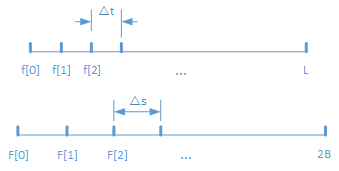
\includegraphics[width=0.4\textwidth]{assets/DFT3.png}
\end{figure}

有$N\cdot\Delta t=L$,$L$为时间上的限制;$N\cdot \Delta s=2\cdot B$,$2\cdot B$为带宽限制:
$$
	\Delta t\cdot \Delta s=\frac{L}{N}\cdot \frac{2\cdot B}{N}=\frac{2\cdot B\cdot L}{N^2}=\frac{N}{N\cdot N}=\frac{1}{N}
$$

时域的采样间隔和频域的采样间隔会根据抽样点数成倒数关系。这该关系对于进行离散 傅立叶变换很有现实意义。

当我们确定好时域的采样间隔$\Delta t$与抽样点数$N$时,频域的采样间隔$\Delta s$就被固定了,即频域分辨率是由时域所做的选择而确定的。
\subsection{引入新符号}

令$\underline{\omega}$为离散的复指数信号(或为复指数向量),且:
\begin{align*}
	\underline{\omega}    & =(1,e^{-2\cdot \pi\cdot i\cdot\frac{1}{N}},e^{-2\cdot \pi\cdot i\cdot\frac{2}{N}},\cdots,e^{-2\cdot \pi\cdot i\cdot\frac{N-1}{N}}) \\
	\underline{\omega}[m] & =e^{-2\cdot \pi\cdot i\cdot\frac{m}{N}}
\end{align*}

那么对$\underline{\omega}$进行幂运算,有:
\begin{align*}
	  & \underline{\omega}^n                                                                                                                                 \\
	= & (1,e^{-2\cdot \pi\cdot i\cdot\frac{n}{N}},e^{-2\cdot \pi\cdot i\cdot\frac{2\cdot n}{N}},\cdots,e^{-2\cdot \pi\cdot i\cdot\frac{(N-1)\cdot n}{N}})    \\
	  & \underline{\omega}^{-n}                                                                                                                              \\
	= & (1,e^{-2\cdot \pi\cdot i\cdot\frac{-n}{N}},e^{-2\cdot \pi\cdot i\cdot\frac{-2\cdot n}{N}},\cdots,e^{-2\cdot \pi\cdot i\cdot\frac{-(N-1)\cdot n}{N}}) \\
	  & \underline{\omega}^{-n}[m] =  e^{-2\cdot \pi\cdot i\cdot\frac{-m\cdot n}{N}}
\end{align*}

把它代入到离散 傅立叶变换中,则有:
$$
	\underline{\mathcal{F}f}[m]=\sum\limits_{n=0}^{N-1}\ \underline{f}[n]\cdot e^{-2\cdot \pi\cdot i\cdot\frac{m\cdot n}{N}}=\sum\limits_{n=0}^{N-1}\ \underline{f}[n]\cdot \underline{\omega}^{-n}[m]
$$

隐藏序号$m$,有:
\begin{equation}
	\underline{\mathcal{F}f}=\sum\limits_{n=0}^{N-1}\ \underline{f}[n]\cdot \underline{\omega}^{-n}
\end{equation}
\section{离散 傅立叶变换特性}
\subsection{输入和输出的周期性}
离散傅立叶变换的定义迫使我们把输入$\underline{f}$与输出$\underline{\mathcal{F}f}$不仅当作定义在$0$到$N-1$整数上的,并且是周期为$N$的周期离散函数。周期性在后面证明。


\subsection{离散复指数的正交性}
%TODO:在普通的傅立叶变换中的复指数也是有正交性
\begin{align*}
	\underline{\omega}   & =(1,e^{-2\cdot \pi\cdot i\cdot\frac{1}{N}},e^{-2\cdot \pi\cdot i\cdot\frac{2}{N}},\cdots,e^{-2\cdot \pi\cdot i\cdot\frac{N-1}{N}})                 \\
	\underline{\omega}^n & =(1,e^{-2\cdot \pi\cdot i\cdot\frac{n}{N}},e^{-2\cdot \pi\cdot i\cdot\frac{2\cdot n}{N}},\cdots,e^{-2\cdot \pi\cdot i\cdot\frac{(N-1)\cdot n}{N}}) \\
\end{align*}

如果$k\neq l$,则有$\underline{\omega}^k$与$\underline{\omega}^l$是正交的。
这里不把$\underline{\omega}$当作离散信号,而是把它当作$N$维向量,我们在讨论傅立叶级数复指数的时候引入了正交,这里可谓是它的离散版本,即:

如果$k\neq l$:
\begin{align*}
	  & \underline{\omega}^k\cdot \underline{\omega}^l                                                                                       \\
	= & \sum\limits_{n=0}^{N-1}\ \underline{\omega}^k[n]\cdot \overline{\underline{\omega}^l[n]}                                             \\
	= & \sum\limits_{n=0}^{N-1}\ e^{2\cdot \pi\cdot i\cdot \frac{k\cdot n}{N}}\cdot \overline{e^{2\cdot \pi\cdot i\cdot \frac{l\cdot n}{N}}} \\
	= & \sum\limits_{n=0}^{N-1}\ e^{2\cdot \pi\cdot i\cdot \frac{k\cdot n}{N}}\cdot e^{-2\cdot \pi\cdot i\cdot \frac{l\cdot n}{N}}           \\
	= & \sum\limits_{n=0}^{N-1}\ (e^{2\cdot \pi\cdot i\cdot \frac{k-l}{N}})^n                                                                \\
	= & \frac{1-(e^{2\cdot \pi\cdot i\cdot \frac{k-l}{N}})^n}{1-e^{2\cdot \pi\cdot i\cdot \frac{k-l}{N}}}                                    \\
	= & \frac{1-e^{2\cdot \pi\cdot i\cdot \frac{k-l}{N}}}{1-e^{2\cdot \pi\cdot i\cdot \frac{k-l}{N}}}                                        \\
	= & \frac{1-[i\cdot\sin(2\cdot\pi\cdot(k-l))+\cos(1\cdot\pi\cdot(k-l))]}{1-e^{2\cdot \pi\cdot i\cdot \frac{k-l}{N}}}                     \\
	= & \frac{1-(0+1)}{1-e^{2\cdot \pi\cdot i\cdot \frac{k-l}{N}}}=0
\end{align*}

如果$k=l$:
\begin{align*}
	  & \underline{\omega}^k\cdot \underline{\omega}^l                                          \\
	= & \sum\limits_{n=0}^{N-1}\ \underline{\omega}^k[n]\cdot\overline{\underline{\omega}^l[n]} \\
	= & \sum\limits_{n=0}^{N-1}\ (e^{2\cdot \pi\cdot i\cdot \frac{k-l}{N}})^n                   \\
	= & \sum\limits_{n=0}^{N-1}\ (e^0)^n\quad (k=l)                                             \\
	= & N
\end{align*}
因此:
\begin{equation}
	\underline{\omega}^k\cdot \underline{\omega}^l=
	\begin{cases}
		0\quad & k\neq l \\
		N\quad & k=l
	\end{cases}
\end{equation}

当$l\neq k$时,$\underline{\omega}^k$与$\underline{\omega}^l$是正交的,但是他们并不是标准正交,因为$\Vert \underline{\omega}^k\Vert=\underline{\omega}^k\cdot \underline{\omega}^k=N$而不是$1$.因此右式为了归一化为标准正交向量,会把$N$引入到$\underline{\omega}$中。
\section{离散傅立叶逆变换}

离散傅立叶逆变换有公式如下:
\begin{equation}
	\underline{\mathcal{F}^{-1}f}[m] = \displaystyle{ \frac{1}{N}\sum_{n=0}^{N-1}\underline{f}[n]e^{2\pi i \frac{mn}{N}} = \frac{1}{N}\sum_{n=0}^{N-1}\underline{f}[n]\underline{\omega}^n[m] }
\end{equation}

省略序号$m$,有:
\begin{equation}
	\underline{\mathcal{F}^{-1}f} = \displaystyle{ \frac{1}{N}\sum_{n=0}^{N-1}\underline{f}[n]\underline{\omega}^n }
\end{equation}

离散傅立叶逆变换的职责是把进行来离散傅立叶变换的离散信号复原,即:
\begin{equation}
	\underline{\mathcal{F}^{-1}\mathcal{F}f} = \underline{f}
\end{equation}
\begin{equation}
	\underline{\mathcal{F}^{-1}\mathcal{F}f}[m] = \underline{f}[m]
\end{equation}

证明过程需要用到$\underline{\omega}$的正交性质:
\begin{align*}
	  & \mathcal{F}^{-1}\mathcal{F}f[m]                                                                                                                                                              \\
	= & \frac{1}{N}\cdot \sum\limits_{n=0}^{N-1}\ \underline{\mathcal{F}f}[n]\cdot e^{2\cdot \pi\cdot i\cdot \frac{m\cdot n}{N}}                                                                     \\
	= & \frac{1}{N}\cdot \sum\limits_{n=0}^{N-1}\ (\sum\limits_{n=0}^{N-1}\ \underline{f}[k]\cdot e^{-2\cdot \pi\cdot i\cdot \frac{k\cdot n}{N}})\cdot e^{2\cdot \pi\cdot i\cdot \frac{m\cdot n}{N}} \\
	= & \frac{1}{N}\cdot \sum\limits_{n=0}^{N-1}\ \underline{f}[k]\cdot (\sum\limits_{n=0}^{N-1}\ e^{-2\cdot \pi\cdot i\cdot \frac{k\cdot n}{N}}\cdot e^{2\cdot \pi\cdot i\cdot \frac{m\cdot n}{N}}) \\
	= & \frac{1}{N}\cdot \sum\limits_{n=0}^{N-1}\ \underline{f}[k]\cdot(\underline{\omega}^k\cdot \underline{\omega}^m)                                                                              \\
	= & \frac{1}{N}\cdot \sum\limits_{n=0}^{N-1}\ \underline{f}[k]\cdot N\quad (\underline{\omega}^k\cdot \underline{\omega}^m=\begin{cases}
		0\quad k\neq m \\
		N\quad k=m
	\end{cases})                                           \\
	= & f[m]
\end{align*}

有$\frac{1}{N}$的原因是,离散复指数是正交的,但不是标准正交的。

\section{离散傅立叶变换的性质}
\subsection{离散傅立叶变换在零点}
$$
	\underline{\mathcal{F}f}(0)=\sum\limits_{n=0}^{N-1}\ \underline{f}[n]\cdot e^{2\cdot \pi\cdot i\cdot \frac{0\cdot n}{N}}=\sum\limits_{n=0}^{N-1}\ \underline{f}[n]
$$

我们可以看到,在零点处的离散傅立叶变换就是是将所有离散信号相加。

类比到傅立叶变换:
$$
	\mathcal{F}f(0)=\int_{-\infty}^\infty\ f(t)\cdot e^{2\cdot \pi\cdot i\cdot 0\cdot t}\ dt=\int_{-\infty}^\infty\ f(t)\ dt
$$
\subsection{典型离散信号}
\subsubsection{$\underline{1}$}
离散信号$\underline{1}$在各个采样点的采样值都为$1$:
$$\underline{1}=(1,1,\cdots,1)$$
\subsubsection{$\underline{\delta_0}$}
$$\underline{\delta_0}=(1,0,\cdots,0)$$

对其进行离散 傅立叶变换:
\begin{align*}
	  & \underline{\mathcal{F}}\underline{\delta_0}                                   \\
	= & \sum\limits_{n=0}^{N-1}\ \underline{\delta_0}[n]\cdot \underline{\omega}^{-n} \\
	= & \underline{\delta_0}[0]\cdot \underline{\omega}^0                             \\
	= & 1\cdot \underline{\omega}^0                                                   \\
	= & (1,1,\cdots,1)=\underline{1}
\end{align*}

因此:
\begin{equation}
	\underline{\mathcal{F}}\underline{\delta_0}=\underline{1}
\end{equation}

\subsubsection{$\underline{\delta_k}$}
$$\underline{\delta_k}=(0,0,\cdots,1,0,\cdots,0)$$

对其进行离散 傅立叶变换:
\begin{align*}
	  & \mathcal{F}\delta_k                                               \\
	= & \sum\limits_{n=0}^{N-1}\ \delta_k[n]\cdot \underline{\omega}^{-n} \\
	= & \underline{\delta_k}[k]\cdot \underline{\omega}^{-k}              \\
	= & 1\cdot \underline{\omega}^{-k}                                    \\
	= & \underline{\omega}^{-k}
\end{align*}
因此:
\begin{equation}
	\underline{\mathcal{F}}\underline{\delta_k}=\underline{\omega}^{-k}
\end{equation}
\subsubsection{$\underline{\omega}^k$}
\begin{align*}
	  & \underline{\mathcal{F}}\underline{\omega}^k[m]                                                                             \\
	= & \sum\limits_{n=0}^{N-1}\ \underline{\omega}^k[n]\cdot \underline{\omega}^{-n}[m]                                           \\
	= & \sum\limits_{n=0}^{N-1}\ e^{2\cdot \pi\cdot i\cdot \frac{k\cdot n}{N}}\cdot e^{-2\cdot \pi\cdot i\cdot \frac{m\cdot n}{N}} \\
	= & \underline{\omega}^k\cdot \underline{\omega}^m                                                                             \\
	= & \begin{cases}
		0 & \ k\neq m \\
		N & \ k=m
	\end{cases}
\end{align*}

因此:
\begin{equation}
	\underline{\mathcal{F}}\underline{\omega}^k=N\cdot \underline{\delta_k}
\end{equation}

\section{离散 傅立叶变换 矩阵}
\subsection{定义}
一般的$\omega$表示为:
$$
	\omega=e^{\frac{-2\cdot\pi}{N}}
$$

离散 傅立叶变换的变换式可以写成:
$$
	\underline{\mathcal{F}f}[m]=\sum\limits_{n=0}^{N-1}\ \omega^{-m\cdot n}\cdot \underline{f}[n]
$$

其中:
$$
	\omega^{-m\cdot n}=e^{-2\cdot \pi\cdot i\cdot \frac{m\cdot n}{N}}
$$

我们换另外一种表示方式:
$$
	\underline{\omega}^{-n}[m]=e^{-2\cdot\pi\cdot\frac{ n\cdot m}{N}}
$$

上式呈现了一种新的表述,即对离散信号$\underline{f}$进行离散 傅立叶变换就相当于用$\underline{f}$与酉矩阵$(\omega^-)^{m\cdot n}$相乘:
\begin{align*}
	      & \left[
		\begin{matrix}
			1      & 1               & 1                     & \cdots & 1                     \\
			1      & \omega^{-1}     & \omega^{-2}           & \cdots & \omega^{-(N-1)}       \\
			1      & \omega^{-2}     & \omega^{-4}           & \cdots & \omega^{-2\cdot(N-1)} \\
			\vdots & \vdots          & \vdots                & \vdots & \vdots                \\
			1      & \omega^{-(N-1)} & \omega^{-2\cdot(N-1)} & \cdots & \omega^{-(N-1)^2}     \\
		\end{matrix}
		\right]        \\
	\cdot &
	\left[
		\begin{matrix}
			\underline{f}[0]   \\
			\underline{f}[1]   \\
			\underline{f}[2]   \\
			\vdots             \\
			\underline{f}[N-1] \\
		\end{matrix}
		\right]
	=  \left[
		\begin{matrix}
			\underline{\mathcal{F}f}[0]   \\
			\underline{\mathcal{F}f}[1]   \\
			\underline{\mathcal{F}f}[2]   \\
			\vdots                        \\
			\underline{\mathcal{F}f}[N-1] \\
		\end{matrix}
		\right]
\end{align*}

上述式子左边的矩阵就是离散 傅立叶变换 矩阵,离散 傅立叶变换 矩阵是一个$N\times N$的酉矩阵,可以用下面的式子表达:
\begin{equation}
	(\mathcal{F})_{m\cdot n}=\omega^{-m\cdot n}
\end{equation}
\subsection{转置共轭与离散傅立叶逆变换矩阵}
对离散傅立叶变换矩阵  $\mathcal{F}$进行共轭转置(酉矩阵的逆矩阵与其伴随矩阵相等),即:

\begin{align*}
	(\mathcal{F}^{*})_{n\times m} = \overline{(\underline{\mathcal{F}})_{m\times n}} = \overline{\omega^{-m\times n}} = \omega^{m\times n}
\end{align*}

离散傅立叶变换矩阵与它的共轭转置矩阵相乘,有:
\begin{align*}
	      & \underline{\mathcal{F}}\cdot \underline{\mathcal{F}}^{*} \\
	=     &
	\left[
		\begin{matrix}
			1      & 1               & 1                & \cdots & 1                 \\
			1      & \omega^{-1}     & \omega^{-2}      & \cdots & \omega^{-(N-1)}   \\
			1      & \omega^{-2}     & \omega^{-4}      & \cdots & \omega^{-2(N-1)}  \\
			\vdots & \vdots          & \vdots           & \cdots & \vdots            \\
			1      & \omega^{-(N-1)} & \omega^{-2(N-1)} & \cdots & \omega^{-(N-1)^2}
		\end{matrix}
		\right]                                                          \\
	\cdot &
	\left[
		\begin{matrix}
			1      & 1              & 1               & \cdots & 1                \\
			1      & \omega^{1}     & \omega^{2}      & \cdots & \omega^{(N-1)}   \\
			1      & \omega^{2}     & \omega^{4}      & \cdots & \omega^{2(N-1)}  \\
			\vdots & \vdots         & \vdots          & \vdots & \vdots           \\
			1      & \omega^{(N-1)} & \omega^{2(N-1)} & \cdots & \omega^{(N-1)^2}
		\end{matrix}
		\right]                                                          \\
	=     & \left[
		\begin{matrix}\underline{\omega}^0\cdot\underline{\omega}^0
			\underline{\omega}^1\cdot\underline{\omega}^0                                                      & \underline{\omega}^2\cdot\underline{\omega}^0     & \cdots & \underline{\omega}^{N-1}\cdot\underline{\omega}^0     \\
			\underline{\omega}^0\cdot\underline{\omega}^1\underline{\omega}^1\cdot\underline{\omega}^1         & \underline{\omega}^2\cdot\underline{\omega}^1     & \cdots & \underline{\omega}^{N-1}\cdot\underline{\omega}^1     \\
			\underline{\omega}^0\cdot\underline{\omega}^2\underline{\omega}^1\cdot\underline{\omega}^2         & \underline{\omega}^2\cdot\underline{\omega}^2     & \cdots & \underline{\omega}^{N-1}\cdot\underline{\omega}^2     \\
			\vdots                                                                                             & \vdots                                            & \vdots & \vdots                                                \\
			\underline{\omega}^0\cdot\underline{\omega}^{N-1}\underline{\omega}^1\cdot\underline{\omega}^{N-1} & \underline{\omega}^2\cdot\underline{\omega}^{N-1} & \cdots & \underline{\omega}^{N-1}\cdot\underline{\omega}^{N-1} \\
		\end{matrix}
		\right]                                                          \\
	=     &
	\left[
		\begin{matrix}
			N      & 0      & 0      & \cdots & 0      \\
			0      & N      & 0      & \cdots & 0      \\
			0      & 0      & N      & \cdots & 0      \\
			\vdots & \vdots & \vdots & \vdots & \vdots \\
			0      & 0      & 0      & \cdots & N
		\end{matrix}
		\right]=N\cdot I
\end{align*}

因此:
\begin{equation}
	\underline{\mathcal{F}}\cdot \underline{\mathcal{F}}^{*}=N\cdot I
\end{equation}

同理:
\begin{equation}
	\underline{\mathcal{F}}^{*}\cdot \underline{\mathcal{F}}=N\cdot I
\end{equation}

通过上面的推导,我们可以可以得到离散傅立叶逆变换矩阵为:
\begin{equation}
	\underline{\mathcal{F}}^{-1} = \frac{1}{N}\underline{\mathcal{F}}^{*}
\end{equation}

即:
\begin{equation}
	\left( \underline{\mathcal{F}}^{-1} \right)_{m\times n} = \frac{1}{N}\omega^{m\times n}
\end{equation}
这个结果同样也能运用推导离散 傅立叶变换矩阵的过程得出。

\subsection{运算复杂度}
这里是指矩阵运算中乘法运算的数目,$\underline{\mathcal{F}f}$的每一项运算会花费$N$个乘法运算,其中共有$N$项,即运算复杂度为$N\times N$,用$O(N^2)$表示。

快速 傅立叶变换算法的目的就是为了减少离散 傅立叶变换的运算复杂度,快速 傅立叶变换的复杂度为$O(NlogN)$。
\section{离散 傅立叶变换特性}
\subsection{输入与输出离散信号周期性的证明}
离散 傅立叶变换的输入和输出都具有均具有周期性,周期为$N$。

如果我们把$\omega$表示在复平面上,它在圆上转圈圈:
\begin{figure}[H]
	\centering
	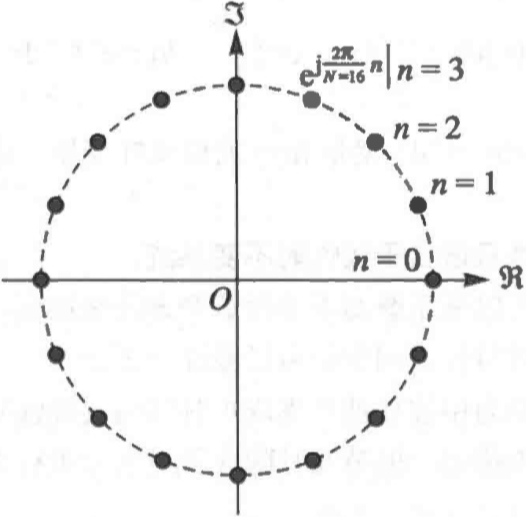
\includegraphics[width=0.4\textwidth]{assets/omega.png}
	\caption{$\omega$的周期性}
\end{figure}

我们取$\underline{\omega}[m] =e^{2\pi i \frac{m}{N}} $。
\subsubsection{离散 傅立叶变换 矩阵中}
\begin{align*}
	  & \underline{\omega}[m+N]               \\
	= & e^{2\pi i\frac{m+N}{N}}               \\
	= & e^{2\pi i\frac{m}{N}}\cdot e^{2\pi i} \\
	= & e^{2\pi i\frac{m}{N}}                 \\
	= & \underline{\omega}[m]                 \\
\end{align*}
同理:
\begin{align*}
	\underline{\omega}^{n}[m]  & = \underline{\omega}^n[m+N]    \\
	\underline{\omega}^{-n}[m] & = \underline{\omega}^{-n}[m+N]
\end{align*}

即$\underline{\omega},\underline{\omega}^n,\underline{\omega}^{-n}$都是周期为$N$的离散复指数信号。


由上述结论推广到离散 傅立叶变换:
\begin{align*}
	  & \underline{\mathcal{F}f}[m+N]                                \\
	= & \sum_{n=0}^{N-1}\underline{f}[n]\underline{\omega}^{-n}[m+N]
	= \sum_{n=0}^{N-1}\underline{f}[n]\underline{\omega}^{-n}[m]     \\
	= & \underline{\mathcal{F}f}[m]
\end{align*}

因此$\underline{\mathcal{F}f}[m+N] = \underline{\mathcal{F}f}[m]$,表明了对离散信号$\underline{f}$进行离散 傅立叶变换后会得到周期为$N$的离散信号。

\subsubsection{离散傅立叶逆变换矩阵}

同理,推广到离散傅立叶逆变换:
\begin{align*}
	  & \underline{\mathcal{F}}^{-1}\underline{f}[m+N]                                                                                                \\
	= & \frac{1}{N}\sum_{n=0}^{N-1}\underline{f}[n]\underline{\omega}^{n}[m+N]= \frac{1}{N}\sum_{n=0}^{N-1}\underline{f}[n]\underline{\omega}^{-n}[m] \\
	= & \underline{\mathcal{F}}^{-1}\underline{f}[m]
\end{align*}

因此$\underline{\mathcal{F}}^{-1}\underline{f}[m+N] = \underline{\mathcal{F}}^{-1}\underline{f}[m]$,表明了对离散信号$\underline{f}$进行离散傅立叶逆变换会得到周期为$N$的离散信号。
\subsubsection{总结}
这种周期为$N$的特性是由$\underline{\omega}$的周期性决定的。对某离散信号$\underline{f}$进行离散 傅立叶变换,会得到周期为$N$的离散信号$\underline{\mathcal{F}f}$,然后对$\underline{\mathcal{F}f}$进行离散傅立叶逆变换,即$\underline{\mathcal{F}^{-1}\mathcal{F}f}$,也会得到周期为$N$的离散信号$\underline{f}$,这表明了原始信号$\underline{f}$也是周期为$N$的离散信号。

因此有结论如下:进行离散 傅立叶变换的输入离散信号$\underline{f}$与输出离散信号$\underline{\mathcal{F}f}$都是周期为$N$($N$项)的周期信号;同理进行离散傅立叶逆变换的输入离散信号$\underline{F}$与输出离散信号$\underline{\mathcal{F}^{-1}\mathcal{F}}$都是周期为$N$($N$项)的周期信号。

% 一开始测量得到的抽样值,必须可以延拓为一系列重复的图像。在离散情况下产生的某些现象,在连续情况下并不存在。原始信号是完全没有周期性的,但是对于有限个测量值的集合情况就不同了。利用傅立叶变换分析,必须使信号具有周期性。在信号没有显示出周期性的情况下,变换会产生周期性。

\subsection{索引的独立性}
周期性可以说是限制,因为我们需要用周期信号来看待将被进行离散 傅立叶变换、I离散 傅立叶变换的离散信号,但是这个特性也带来了简单有益的结论:索引的独立性(independence of indexing)。

由于$\underline{f}$与$\underline{\omega}$都具有周期性,因此在计算离散 傅立叶变换时可以采用任意连续$N$个采样,即:

\begin{align*}
	\underline{\mathcal{F}f} =  \sum_{n=0}^{N-1}\underline{f}[n]\underline{\omega}^{-n} = \sum_{n=1}^{N}\underline{f}[n]\underline{\omega}^{-n}
\end{align*}

我们也可以把零点放置取样值的中间,即:
\begin{align*}
	\underline{\mathcal{F}f} =  \sum_{n=-\frac{N-1}{2}}^{\frac{N-1}{2}}\underline{f}[n]\underline{\omega}^{-n}
\end{align*}

当$N$为奇数时:
\begin{align*}
	\underline{\mathcal{F}f} = \sum_{n=-\frac{N-1}{2}}^{\frac{N-1}{2}}\underline{f}[n]\underline{\omega}^{-n}
\end{align*}

当$N$为偶数时:
\begin{align*}
	\underline{\mathcal{F}f} =  \sum_{n=-\frac{N}{2}+1}^{\frac{N}{2}}\underline{f}[n]\underline{\omega}^{-n}
\end{align*}

在连续的情况下,我们总是考虑对称性,但是在离散的情况下,我们对对称性就没有那么看重了,我们看重的是周期性。
\subsection{离散信号的反转及其离散 傅立叶变换的对偶性}
\subsubsection{离散信号反转的定义}
在讨论连续信号的反转的时候,连续信号$f(x)$的反转为$f^-(x) = f(-x)$,而这里离散信号的反转被定义为$\underline{f}^{-}[m] = \underline{f}[-m]$,也就是说,如果有离散信号:
\begin{align*}
	\underline{f} = \left(\underline{f}[0],\underline{f}[1],\underline{f}[2],\cdots,\underline{f}[N-1] \right)
\end{align*}

它的反转为:
\begin{align*}
	\underline{f}^- = \left( \underline{f}[0],\underline{f}[-1],\underline{f}[-2], \cdots ,\underline{f}[-(N-1)] \right)
\end{align*}

离散复指数$\underline{\omega}$的反转为:
\begin{align*}
	\underline{\omega}^- = \left( 1,e^{-2\pi i\frac{1}{N}},e^{-2\pi i\frac{2}{N}},\cdots,e^{-2\pi i\frac{N-1}{N}} \right) = \underline{\omega}^{-1}
\end{align*}

同理有:
\begin{align*}
	\left(\underline{\omega}^n \right)^-    & = \underline{\omega}^{-n} \\
	\left(\underline{\omega}^{-n} \right)^- & = \underline{\omega}^{n}
\end{align*}
\subsubsection{离散 傅立叶变换对偶性讨论}
对离散信号$\underline{f}$的反转$\underline{f}^-$进行离散 傅立叶变换:
\begin{align*}
	  & \underline{\mathcal{F}f}^-                                                                                \\
	= & \sum_{n=0}^{N-1}\underline{f}^-[n]\underline{\omega}^{-n}                                                 \\
	= & \sum_{n=0}^{N-1}\underline{f}[-n]\underline{\omega}^{-n}    \quad (definition\ of\ reversed\ 信号)        \\
	= & \sum_{n=0}^{N-1}\underline{f}[N-n]\underline{\omega}^{-n}   \quad (\underline{f}\ is\ period\ of\ N)      \\
	= & \sum_{l=N}^1\underline{f}[l]\underline{\omega}^{l-N}        \quad (letting\ l=N-n)                        \\
	= & \sum_{l=N}^1\underline{f}[l]\underline{\omega}^l            \quad (\underline{\omega}\ is\ period\ of\ N) \\
	= & \sum_{l=0}^{N-1}\underline{f}[l]\underline{\omega}^l        \quad (independence\ of\ indexing)            \\
	= & \sum_{l=0}^{N-1}\underline{f}[l](\underline{\omega}^{-l})^-                                               \\
	= & \left(
	\sum_{l=0}^{N-1}\underline{f}[l]\underline{\omega}^{-l} \right )^-                                            \\
	= & \left(\underline{\mathcal{F}f}\right )^-
\end{align*}

因此:
\begin{equation}
	\underline{\mathcal{F}f}^- = \left( \underline{\mathcal{F}f} \right)^-
\end{equation}

对离散信号连续进行两次离散 傅立叶变换:
\begin{align*}
	  & \underline{\mathcal{F}\mathcal{F}f}                                                                                                                                                                         \\
	= & \sum_{k=0}^{N-1}\left(\sum_{n=0}^{N-1}\underline{f}[n]\underline{\omega}^{-n}[k]\right)\underline{\omega}^{-k}                                                                                              \\
	= & \sum_{n=0}^{N-1}\underline{f}[n]\left(\sum_{k=0}^{N-1}\underline{\omega}^{-n}[k]\underline{\omega}^{-k}\right)                                                                                              \\
	= & \sum_{n=0}^{N-1}\underline{f}[n]\left(\underline{\mathcal{F}}\underline{\omega}^{-n}\right)                                                                                                                 \\
	= & \sum_{n=0}^{N-1}\underline{f}[n]\cdot N\underline{\delta_{-n}}                                                                                                                                              \\
	= & N\sum_{n=0}^{N-1}\underline{f}[n]\underline{\delta_{-n}}                                                                                                                                                    \\
	= & N\sum_{n=0}^{N-1}\underline{f}[n]\left(\underline{\delta_n}\right)^-                                                                                                                                        \\
	= & N\left(\sum_{n=0}^{N-1}\underline{f}[n]\underline{\delta_n}\right)^-\qquad\left(\sum_{n=0}^{N-1}\underline{f}[n](\underline{\delta_n})^-[m]=\sum_{n=0}^{N-1}\underline{f}[n]\underline{\delta_n}[-m]\right) \\
	= & N\left(\sum_{n=0}^{N-1}\underline{f}[n]\underline{\delta_n}[0],\sum_{n=0}^{N-1}\underline{f}[n]\underline{\delta_n}[1],\cdots,\sum_{n=0}^{N-1}\underline{f}[n]\underline{\delta_n}[N-1]\right)^-
\end{align*}

我们来分析一下$\sum_{n=0}^{N-1}\underline{f}[n]\underline{\delta_n}[0]$,其中:
$$
	\underline{\delta_n}[m]=\begin{cases} 1 & \quad m=n     \\
		0 & \quad m\neq n\end{cases}
$$

因此:

\begin{align*}
	  & \underline{\mathcal{F}\mathcal{F}f}                                                                                      \\
	= & N\cdot (\sum_{n=0}^{N-1}\underline{f}[n]\underline{\delta_n}[0],\sum_{n=0}^{N-1}\underline{f}[n]\underline{\delta_n}[1], \\
	  & \cdots,\sum_{n=0}^{N-1}\underline{f}[n]\underline{\delta_n}[N-1])^-                                                      \\
	= & N\cdot (\underline{f}[0],\underline{f}[1],\cdots,\underline{f}[N-1])^-                                                   \\
	= & N\underline{f}^-
\end{align*}

最终得:
\begin{equation}
	\underline{\mathcal{F}\mathcal{F}f} = N\cdot \underline{f}^-
\end{equation}

\section{快速傅立叶变换}
离散傅立叶变换矩阵运算中主要的计算量(乘法计算量)为$N \times N$,用$O(N^2)$表示,而快速 傅立叶变换可以将计算量降到$N\cdot \log{N}$。
\subsection{矩阵简化}
\subsubsection{复数矩阵}
\begin{enumerate}
	\item H
	      \begin{equation}
		      \overline{\vec{z}}^T=\vec{z}^H
	      \end{equation}
	\item 酉矩阵

	      我们这样定义标准正交向量:
	      $$
		      q_i^Tq_j=\begin{cases}0\quad i\neq j\\1\quad i=j\end{cases}
	      $$

	      现在,对于复向量我们需要求共轭:
	      $$
		      \bar{q}_i^Tq_j=q_i^Hq_j=\begin{cases}0\quad i\neq j\\1\quad i=j\end{cases}
	      $$

	      标准正交矩阵:
	      $
		      Q=\Bigg[q_1\ q_2\ \cdots\ q_n\Bigg]
	      $
	      有:$Q^TQ=I$;现在对于复矩阵则有:$Q^HQ=I$。

	      正交性(orthogonal)在复数情况下也有了新名字,酉(unitary),酉矩阵(unitary matrix)与正交矩阵类似,满足$Q^HQ=I$的性质。而前面提到的傅里叶矩阵就是一个酉矩阵。
\end{enumerate}
\subsubsection{傅里叶矩阵}
\begin{align*}
	F_n=\begin{bmatrix}1&1&1&\cdots&1\\1&\omega &\omega ^2&\cdots&\omega ^{N-1}\\1&\omega ^2&\omega ^4&\cdots&\omega ^{2(N-1)}\\\vdots&\vdots&\vdots&\ddots&\vdots\\1&\omega ^{N-1}&\omega ^{2(N-1)}&\cdots&\omega ^{(N-1)^2}\end{bmatrix}
\end{align*}

对于每一个元素有:
\begin{equation}
	(F_N)_{ij}=\omega ^{i\times j}\quad i,j=0,1,2,\cdots,N-1
\end{equation}

矩阵中的$\omega=e^{\frac{2\cdot \pi\cdot i}{N}}$满足:$\omega ^N=1$。

易知在复平面的单位圆上,$\omega=\cos\frac{2\cdot \pi}{N}+i\cdot \sin\frac{2\cdot \pi}{N}$。

在傅里叶矩阵中,当我们计算$\omega$的幂时,$\omega$在单位圆上的角度翻倍。
比如在$6$阶情形下,$\omega=e^{i\cdot 2\cdot \pi/6}$,即位于单位圆上$60^\circ$角处,其平方位于单位圆上$120^\circ$角处,而$\omega$位于$1$处。从开方的角度看,它们是$1$的$6$个六次方根,而一次的$\omega$称为原根。

我们以研究$4$阶的傅立叶矩阵为例。先计算$\omega$,有$\omega=i$,$\omega^2=-1$,$\omega^3=-i$,$\omega^4=1$:
\begin{align*}
	F_4=\begin{bmatrix}1&1&1&1\\1&i&i^2&i^3\\1&i^2&i^4&i^6\\1&i^3&i^6&i^9\end{bmatrix}=\begin{bmatrix}1&1&1&1\\1&i&-1&-i\\1&-1&1&-1\\1&-i&-1&i\end{bmatrix}
\end{align*}

矩阵的四个列向量正交,不过我们应该注意到,$F_4$的列向量并不是标准的,我们可以给矩阵乘上系数$\frac{1}{2}$(除以列向量的长度)得到标准正交矩阵:
\begin{align*}
	F_4=\frac{1}{2}\cdot \begin{bmatrix}1&1&1&1\\1&i&-1&-i\\1&-1&1&-1\\1&-i&-1&i\end{bmatrix}
\end{align*}

此时有$F_4^HF_4=I$,于是该矩阵的逆矩阵也就是其共轭转置$F_4^H$。

我们来分解$F_{64}$这个式子。我们可以发现$F_{64}^2=F_{32}$。
\begin{align*}
	\Bigg[F_{64}\Bigg]=\begin{bmatrix}
		I & D \\I&-D
	\end{bmatrix}
	\cdot
	\begin{bmatrix}F_{32}&0\\0&F_{32}\end{bmatrix} \\
	\cdot
	\begin{bmatrix}
		1 & \quad & \cdots & \quad  & \quad & 0     & \quad & \cdots & \quad  & \quad \\
		0 & \quad & \cdots & \quad  & \quad & 1     & \quad & \cdots & \quad  & \quad \\
		  & 1     & \quad  & \cdots & \quad & \quad & 0     & \cdots & \quad  & \quad \\
		  & 0     & \quad  & \cdots & \quad & \quad & 1     & \cdots & \quad  & \quad \\
		  & \quad & \quad  & \ddots & \quad & \quad & \quad & \quad  & \ddots & \quad \\
		  & \quad & \quad  & \ddots & \quad & \quad & \quad & \quad  & \ddots & \quad \\
		  & \quad & \quad  & \cdots & 1     & \quad & \quad & \quad  & \cdots & 0     \\
		  & \quad & \quad  & \cdots & 0     & \quad & \quad & \quad  & \cdots & 1
	\end{bmatrix}
\end{align*}

我们分开来看等式右侧的这三个矩阵:
\begin{enumerate}
	\item 第一个矩阵由单位矩阵$I$和对角矩阵$D=\begin{bmatrix}1&&&&\\&w&&&\\&&w^2&&\\&&&\ddots&\\&&&&w^{31}\end{bmatrix}$组成。我们称这个矩阵为修正矩阵,显然其计算量来自$D$矩阵。
	\item 第二个矩阵为两个$F_{32}$与零矩阵组成的。
	\item 第三个矩阵通常记为$P$矩阵,这是一个置换矩阵,其作用是讲前一个矩阵中的奇数列提到偶数列之前,将前一个矩阵从$\Bigg[x_0\ x_1\ \cdots\Bigg]$,变为$\Bigg[x_0\ x_2\ \cdots\ x_1\ x_3\ \cdots\Bigg]$。
\end{enumerate}

\subsection{利用复指数的代数性质}
我们把和写成一个分成奇偶指数的和的形式。我们试着把一个$N$阶的离散 傅立叶变换转换成两个$\frac{N}{2}$阶离散 傅立叶变换的组合。

要做到这一点,你需要假设$N$是偶数;为了继续迭代分解(iterate),你需要假设$N$是$2$的乘方。
\subsubsection{引入$\omega[p,q]$}
令$\omega[p,q] = e^{2\pi i\frac{q}{p}}$,则:
\begin{align*}
	  & \omega[p,q_1+q_2]                \\
	= & e^{2\pi i\frac{q_1+q_2}{p}}      \\
	= & \omega[p,q_1]\cdot \omega[p,q_2]
\end{align*}

那么:
\begin{align*}
	  & \omega[\frac{N}{2},-n\cdot m]                             \\
	= & e^{2\cdot \pi\cdot  i\cdot \frac{-n\cdot m}{\frac{N}{2}}} \\
	= & \omega[N,-2\cdot n\cdot m]
\end{align*}

这表明了$\omega[\frac{N}{2},-1]$是$\omega[N,-1]$的偶次方。

等式右边的$2\cdot n$代表了偶次方,那么$\omega[N,-1]$的奇次方呢?
\begin{align*}
	  & \omega[N,-(2\cdot n+1)\cdot m]                  \\
	= & \omega[N,-2\cdot n\cdot m-m]                    \\
	= & \omega[N,-2\cdot n\cdot m]\cdot    \omega[N, m] \\
	= & \omega[\frac{N}{2},-n\cdot m]\cdot \omega[N,-m]
\end{align*}

总结一下,有:
\begin{equation}
	\omega[N,-2\cdot n\cdot m]  = \omega[\frac{N}{2},-n\cdot m]
\end{equation}
\begin{equation}
	\omega[N,-(2\cdot n+1)\cdot m]  = \omega[N,-m]\cdot \omega[\frac{N}{2},-n\cdot m]
\end{equation}

\subsubsection{把离散傅立叶变换公式表达成奇偶项的形式}
接下来就是把上述关于$\omega$的奇偶等式代入到离散 傅立叶变换公式。

首先来回顾一下离散 傅立叶变换公式:
$$
	\underline{\mathcal{F}f}[m] =  \sum_{n=0}^{N-1}\underline{f}[n]\omega[N,-n\cdot m]
$$

式子当中共有$N$项多项式相加,我们需要把这$N$项多项式分为奇数与偶数部分,即:
\begin{align*}
	  & \underline{\mathcal{F}f}[m]                          \\
	= & (sum\ over\ even\ indices)+(sum\ over\ odd\ indices)
\end{align*}

但是$N$可能不是偶数,这会导致分出来的奇偶项的数目不等,这不符合我们后续的推导过程,因此我们会假设$N$为偶数,即可以按下面的式子进行划分:
\begin{align*}
	  & \underline{\mathcal{F}f}[m]                                                       \\
	= & \sum_{n=0}^{\frac{N}{2}-1}\underline{f}[2n]\omega[N,-2\cdot n\cdot m]             \\
	+ & \sum_{n=0}^{\frac{N}{2}-1}\underline{f}[2\cdot n+1]\omega[N,-(2\cdot n+1)\cdot m]
\end{align*}

我们后面会继续按照这种奇偶项的分解方法一直进行下去,这就要求$N$必须为2的某次方($N=2^k$),但是在实际的离散 傅立叶变换应用中,可能会出现$N$不为$2^k$的情况,在这种情况下我们就需要在后面补$0$。
\begin{align*}
	\underline{f} = (\underbrace{ \underline{f}[0],\underline{f}[1],\cdots,\underline{f}[N-1],0,0,\cdots,0 }_{2^k\ entries} )
\end{align*}

有了上述条件,我们回到离散 傅立叶变换公式的分解推导,
\begin{align*}
	  & \underline{\mathcal{F}f}                                                                                 \\
	= & \sum_{n=0}^{\frac{N}{2}-1}\underline{f}[2\cdot n]\cdot \omega[N,-2\cdot n\cdot m]                        \\
	+ & \sum_{n=0}^{\frac{N}{2}-1}\underline{f}[2\cdot n+1]\cdot \omega[N,-(2\cdot n+1)\cdot m]                  \\
	= & \sum_{n=0}^{\frac{N}{2}-1}\underline{f}[2\cdot n]\cdot \omega[\frac{N}{2},-n\cdot m]                     \\
	+ & \sum_{n=0}^{\frac{N}{2}-1}\underline{f}[2\cdot n+1]\cdot \omega[N,-m]\cdot \omega[\frac{N}{2},-n\cdot m] \\
	= & \sum_{n=0}^{\frac{N}{2}-1}\underline{f}[2\cdot n]\cdot \omega[\frac{N}{2},-n\cdot m]                     \\
	+ & \omega[N,-m]\sum_{n=0}^{\frac{N}{2}-1}\underline{f}[2\cdot n+1]\omega[\frac{N}{2},-n\cdot m]
\end{align*}

我们来分析一下上述推导结果,上式的奇偶两个大项,基本上可以被当作单独的离散 傅立叶变换。其中:
\begin{enumerate}
	\item 每个大项的离散数据有$\frac{N}{2}$个;
	\item 求和从$0$到$\frac{N}{2}-1$;
	\item $\omega[\frac{N}{2},-n\cdot m] = e^{-2\pi i\frac{n\cdot m}{\frac{N}{2}}}$中的复指数分母也由$N$替换成了$\frac{N}{2}$。
\end{enumerate}

但是其中还有一点瑕疵,因为离散傅立叶变换是有多少个输入就会有多少个输出:$\underline{f}$有$N$个输入,则$\underline{\mathcal{F}f}$有$N$个输出,也就是说$m =0,1,\cdots,N-1$;但是$\sum\limits_{n=0}^{\frac{N}{2}-1}\underline{f}[2\cdot n]\omega[\frac{N}{2},-n\cdot m]$只有$\frac{N}{2}$个输入,也只应该有$\frac{N}{2}$个输出,也就是说$m= 0,1,\cdots,\frac{N}{2}-1$,这就与原来的离散 傅立叶变换定义相悖了。因此我们可以遵照以下规定:
\begin{align*}
	  & \underline{\mathcal{F}_N f}[m]                                                                                                             \\
	= & \left( \underline{\mathcal{F}_{\frac{N}{2}}f}_{even} \right)[m]+\omega[N,-m]\left( \underline{\mathcal{F}_{\frac{N}{2}}f}_{odd} \right)[m] \\
	  & (m=0,1, \cdots,\frac{N}{2})
\end{align*}
这样的话只处理了$\underline{\mathcal{F}f}$的前半部分,那后半部分该怎么表达呢?

后半部分的输出个数还是为$\frac{N}{2}$:
\begin{enumerate}
	\item $\underline{\mathcal{F}f}[m]$,变成$\underline{\mathcal{F}f}[m+\frac{N}{2}]$,$m = 0,1,\cdots,\frac{N}{2}-1$。
	\item $\sum\limits_{n=0}^{\frac{N}{2}-1}$与$\underline{f}[2\cdot n]$、$\underline{f}[2\cdot n+1]$,不涉及到$m$,不变;
	\item $\omega[\frac{N}{2},-n\cdot m]$,变成$\omega[\frac{N}{2},-n\cdot (m+\frac{N}{2})] = \omega[\frac{N}{2},-n\cdot m]\cdot \omega[\frac{N}{2},-\frac{N}{2}\cdot n] = \omega[\frac{N}{2},-n\cdot m]$,相当于不变;
	\item $\omega[N,-m]$,变成$\omega[N,-(m+\frac{N}{2})] = \omega[N,-m]\cdot \omega[N,-\frac{N}{2}] = \omega[N,-m]$,也就是多了个负号。
\end{enumerate}

把上述变化统合起来,有
\begin{align*}
	  & \underline{\mathcal{F}f}[m+\frac{N}{2}]                                                                       \\
	= & \sum_{n=0}^{\frac{N}{2}-1}\underline{f}[2\cdot n]\cdot \omega[\frac{N}{2},-n\cdot m]                          \\
	- & \omega[N,-m]\cdot \sum_{n=}^{\frac{N}{2}-1}\cdot \underline{f}[2\cdot n+1]\cdot \omega[\frac{N}{2},-n\cdot m]
\end{align*}

即:
\begin{align*}
	  & \underline{\mathcal{F}}_N\underline{f}[m]                                                                                                                          \\
	= & \left( \underline{\mathcal{F}}_{\frac{N}{2}}\underline{f}_{even} \right)[m]-\omega[N,-m]\left( \underline{\mathcal{F}}_{\frac{N}{2}}\underline{f}_{odd} \right)[m] \\
	  & (m=0,1, \cdots,\frac{N}{2})
\end{align*}
\subsection{总结}
有$N$元输入的离散信号$\underline{f}$(其中$N=2^k$),我们想推导它的$N$元输出$\underline{\mathcal{F}f}$。我们把需要得到的$\underline{\mathcal{F}f}$分为前后两半,前半的各项为$\underline{\mathcal{F}f}[m]$,后半各项为$\underline{\mathcal{F}f}[m+\frac{N}{2}]$,$m=0,1,\cdots,\frac{N}{2}-1$

计算步骤如下:
\begin{enumerate}
	\item 把输入$\underline{f}$分成偶数与奇数两个序列$\underline{f}_{even}$,$\underline{f}_{odd}$;
	\item 把$\underline{f}_{even}$,$\underline{f}_{odd}$当作单一的输入,分别计算他们的$\underline{\mathcal{F}}_{\frac{N}{2}}\underline{f}_{even}$,$\underline{\mathcal{F}}_{\frac{N}{2}}\underline{f}_{odd}$;
	\item 通过把$\underline{\mathcal{F}}_{\frac{N}{2}}\underline{f}_{even}$,$\underline{\mathcal{F}}_{\frac{N}{2}}\underline{f}_{odd}$按照下列式子的方式结合起来,可以分别得到$\underline{\mathcal{F}f}$的前后半部分:

	      \begin{align*}
		      \underline{\mathcal{F}}_N\underline{f}[m] & = \left( \underline{\mathcal{F}}_{\frac{N}{2}}\underline{f}_{even} \right)[m]+\omega[N,-m]\left( \underline{\mathcal{F}}_{\frac{N}{2}}\underline{f}_{odd} \right)[m] \\
		      \underline{\mathcal{F}}_N\underline{f}[m] & = \left( \underline{\mathcal{F}}_{\frac{N}{2}}\underline{f}_{even} \right)[m]-\omega[N,-m]\left( \underline{\mathcal{F}}_{\frac{N}{2}}\underline{f}_{odd} \right)[m] \\
		      \omega[N,-m]                              & = e^{-2\pi i\frac{m}{N}}\quad (m=0,1,\cdots,\frac{N}{2}-1)
	      \end{align*}
\end{enumerate}


前文推导出的这段计算虽然不能算快速 傅立叶变换的全貌,却包含了快速 傅立叶变换的主要思想:把一个完整的离散 傅立叶变换二分成偶数项$\underline{f}_{even}$以及奇数项$\underline{f}_{odd}$的离散 傅立叶变换的组合,然后又再继续对$\underline{f}_{even}$与$\underline{f}_{odd}$继续二分,直到最终剩下两项。
\begin{figure}[H]
	\centering
	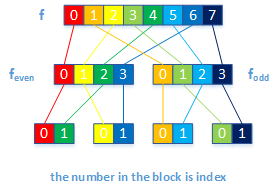
\includegraphics[width=0.4\textwidth]{assets/FFT.png}
\end{figure}

\end{document}